\documentclass[12pt,a4paper]{report}

% ─── Pakete ────────────────────────────────────────────────────────────────────
\usepackage[utf8]{inputenc}
\usepackage[T1]{fontenc}
\usepackage[ngerman]{babel}
\usepackage{geometry}

\usepackage{amsmath, amssymb, amsthm, mathtools}
\usepackage{graphicx}
\usepackage{booktabs}
\usepackage{array}
\usepackage{longtable}
\usepackage{hyperref}
\usepackage{xcolor}
\usepackage{enumitem}
\usepackage{setspace}
\usepackage{caption}
\captionsetup{width=\linewidth, singlelinecheck=false}
\usepackage{fancyhdr}
\usepackage{parskip}
\usepackage{microtype}

\usepackage{textcomp}  % für \texteuro
\usepackage{tikz}
\usetikzlibrary{arrows.meta, positioning, shapes.geometric, fit, backgrounds}

\setlist[itemize,1]{label=--}

% ─── Layout ────────────────────────────────────────────────────────────────────
\geometry{margin=2.5cm, headheight=15pt}

\hypersetup{colorlinks=true, linkcolor=[rgb]{0.0,0.3,0.6},
	citecolor=[rgb]{0.0,0.3,0.6}, urlcolor=[rgb]{0.0,0.3,0.6}}

% ─── Theorem-Umgebungen ────────────────────────────────────────────────────────
\theoremstyle{plain}
\newtheorem{theorem}{Theorem}[section]
\newtheorem{lemma}[theorem]{Lemma}
\newtheorem{korollar}[theorem]{Korollar}
\newtheorem{proposition}[theorem]{Proposition}

\theoremstyle{definition}
\newtheorem{definition}[theorem]{Definition}
\newtheorem{experiment}[theorem]{Experiment}
\newtheorem{axiom}[theorem]{Axiom}
\newtheorem{beobachtung}[theorem]{Beobachtung}

\theoremstyle{remark}
\newtheorem{bemerkung}[theorem]{Bemerkung}
\newtheorem{beispiel}[theorem]{Beispiel}

% ─── Mathe-Operatoren ──────────────────────────────────────────────────────────
\DeclareMathOperator{\GHI}{GHI}
\DeclareMathOperator{\BRK}{BRK}
\DeclareMathOperator{\SGN}{sgn}
\DeclareMathOperator{\EMG}{EMG}
\DeclareMathOperator{\GRF}{GRF}

% Subskript-Hilfsmakros
\newcommand{\med}{\mathrm{med}}  % G_{\med} – M. gluteus medius
\newcommand{\euro}{\texteuro}    % Euro-Zeichen

% ══════════════════════════════════════════════════════════════════════════════
\title{\textbf{Die Notwendigkeit eines gesunden Hinterns}\\[0.4em]
	\large Eine biomechanische, neuromotorische und physiologische\\
	Formalisierung des Gluteus-Grundsatzes}
\author{Stephan Epp}
\date{16. März 2026}

% ══════════════════════════════════════════════════════════════════════════════
\begin{document}
	\maketitle
	
	\tableofcontents
	\newpage
	
	% ══════════════════════════════════════════════════════════════════════════════
	\chapter{Einleitung}
	% ══════════════════════════════════════════════════════════════════════════════
	Die vorliegende Arbeit entwickelt und beweist formal den \emph{Gluteus-Grundsatz}:
	Ein strukturell und funktionell gesundes Gesäß -- insbesondere der
	\emph{Musculus gluteus maximus} sowie seine synergistischen Begleitstrukturen --
	ist eine notwendige Bedingung für posturale Stabilität, effiziente Lokomotion,
	lumbale Gesundheit und langfristige muskuloskelettale Integrität des Menschen.
	Wir formalisieren diese Notwendigkeit in einem vierdimensionalen Funktionsrahmen,
	beweisen Existenz und Eindeutigkeit des biomechanischen Gleichgewichts,
	analysieren die Atrophiedynamik als Differentialgleichungssystem und
	leiten das optimale Trainingsprogramm mittels Variationsrechnung her.
	Zehn quantitative Analysen mit numerischen Simulationen und
	epidemiologischen Modellen belegen die Aussagen.
	
	Der menschliche Körper ist ein hochoptimiertes mechanisches System, dessen
	evolutionäre Entwicklung über Millionen von Jahren auf aufrechten, aktiven
	Zweibeingang ausgerichtet war. Im Zentrum dieser Optimierung steht eine
	anatomische Struktur, die im gesellschaftlichen Diskurs häufig unterschätzt wird:
	das Gesäß. Genauer gesagt ist der \emph{Musculus gluteus maximus}
	-- der größte Muskel des menschlichen Körpers -- zusammen mit den synergistisch
	wirkenden \emph{Mm. glutei medius et minimus} der primäre Stabilisator des
	Hüftgelenks, der Lendenwirbelsäule und des gesamten posturalen Systems.
	
	Die Industrialisierung und die damit einhergehende sitzende Lebensweise haben
	zu einer systematischen Atrophie dieser muskulären Grundstruktur geführt.
	Fachleute sprechen von \emph{glutealer Amnesie} -- einem Zustand, in dem
	das zentralnervöse System die korrekte Aktivierungssequenz der Glutealmuskulatur
	nicht mehr abrufen kann. Die Konsequenzen sind vielfältig und weitreichend:
	chronische Rückenschmerzen, Knie- und Hüftarthrose, Gangstörungen,
	erhöhtes Sturzrisiko im Alter sowie eine reduzierte Energieeffizienz
	bei sämtlichen motorischen Aufgaben.
	
	Die vorliegende Arbeit verfolgt das Ziel, die \emph{Notwendigkeit} eines
	gesunden Gesäßes nicht allein qualitativ zu beschreiben, sondern formal
	nachzuweisen. Wir formulieren den zentralen \emph{Gluteus-Grundsatz}
	als mathematische Aussage und führen seinen Beweis auf biomechanischer,
	regelungstechnischer und variationsrechnerischer Ebene.
	
	\section{Zielsetzung und Aufbau}
	
	Die Arbeit gliedert sich wie folgt:
	Kapitel~\ref{chap:anatomie} legt die anatomischen und physiologischen Grundlagen.
	Kapitel~\ref{chap:formalisierung} führt den formalen Rahmen ein und definiert
	den Gluteus-Gesundheitsindex $\GHI$.
	Kapitel~\ref{chap:biomechanik} analysiert die biomechanischen Implikationen
	-- Druckverteilung, Hebelmodell, Wirbelsäulenbelastung.
	Kapitel~\ref{chap:dynamik} behandelt die Atrophiedynamik als ODE-System.
	Kapitel~\ref{chap:gang} untersucht den Einfluss auf Gangbild und Stabilität.
	Kapitel~\ref{chap:energie} quantifiziert die energetische Bedeutung.
	Kapitel~\ref{chap:regelung} modelliert die posturale Regelung als Regelkreis.
	Kapitel~\ref{chap:epidemiologie} präsentiert epidemiologische Evidenz.
	Kapitel~\ref{chap:optimierung} leitet das optimale Trainingsprogramm her.
	Kapitel~\ref{chap:zusammenfassung} fasst die Ergebnisse zusammen.
	
	% ══════════════════════════════════════════════════════════════════════════════
	\chapter{Anatomische und physiologische Grundlagen}
	\label{chap:anatomie}
	% ══════════════════════════════════════════════════════════════════════════════
	
	\section{Die Glutealmuskulatur}
	
	Das Gesäß im funktionellen Sinne umfasst drei Hauptmuskeln:
	
	\begin{definition}[Glutealtriade]
		Die \emph{Glutealtriade} $\mathcal{G} = (G_{\max}, G_{\med}, G_{\min})$
		bezeichnet die funktionelle Einheit aus
		\[
		G_{\max} := \text{M. gluteus maximus},
		G_{\med} := \text{M. gluteus medius},
		G_{\min} := \text{M. gluteus minimus.}
		\]
		Ihre kombinierte Kraft- und Stabilitätswirkung konstituiert das
		\emph{gluteale Funktionssystem} $\Gamma$.
	\end{definition}
	
	Der \emph{M. gluteus maximus} ist der größte und stärkste Muskel des
	menschlichen Körpers. Seine physiologischer Querschnitt beträgt beim
	trainierten Erwachsenen bis zu $50\,\mathrm{cm}^2$,
	sein Kraftpotenzial liegt bei $800$--$1800\,\mathrm{N}$
	je nach Trainingszustand. Primäre Funktion ist die Hüftextension,
	Außenrotation und Abduktion.
	
	Der \emph{M. gluteus medius} und \emph{minimus} stabilisieren das Becken
	in der Frontalebene -- sie verhindern das \emph{Trendelenburg-Zeichen},
	das Abkippen des Beckens zur Standbeinseite, und sind essenziell
	für einen physiologischen Gang.
	
	\section{Funktionelle Relevanz}
	
	\begin{axiom}[Posturales Primärprinzip]
		\label{ax:postural}
		Jede aufrechte Haltung und jede Lokomotionsform des Menschen erfordert
		die koordinierte Aktivierung mindestens eines Elements der Glutealtriade $\mathcal{G}$.
	\end{axiom}
	
	Axiom~\ref{ax:postural} ist anatomisch fundiert: Das Hüftgelenk als zentrales
	Gelenk zwischen Rumpf und unterer Extremität wird primär durch die
	Glutealmuskulatur stabilisiert. Alle anderen Strukturen -- Hüftbeuger,
	Ischiokrurale, Kniestrecker -- können diese Funktion nur partiell und
	ineffizient kompensieren.
	
	% ══════════════════════════════════════════════════════════════════════════════
	\chapter{Formaler Rahmen und der Gluteus-Grundsatz}
	\label{chap:formalisierung}
	% ══════════════════════════════════════════════════════════════════════════════
	
	\section{Der Gluteus-Gesundheitsindex}
	
	\begin{definition}[Gluteus-Gesundheitsindex $\GHI$]
		\label{def:ghi}
		Sei $M(t) \geq 0$ der physiologische Muskelquerschnitt des M. gluteus maximus
		zum Zeitpunkt $t$, $\eta(t) \in [0,1]$ seine neuromuskuläre Aktivierungseffizienz,
		und $\kappa(t) \in [0,1]$ der Koordinationsindex der Glutealtriade. Der
		\emph{Gluteus-Gesundheitsindex} ist definiert als
		\[
		\GHI(t) := \frac{M(t) \cdot \eta(t) \cdot \kappa(t)}{M_0 \cdot \eta_0 \cdot \kappa_0}
		\in [0,1],
		\]
		wobei $M_0,\eta_0,\kappa_0$ die Referenzwerte einer gesunden, trainierten
		Vergleichspopulation bezeichnen.
	\end{definition}
	
	\begin{definition}[Gesundes Gesäß]
		\label{def:gesund}
		Ein Gesäß heißt \emph{gesund} im Sinne dieser Arbeit, wenn
		\[
		\GHI(t) \geq \GHI_{\min} := 0{,}65 \quad \forall t \in [t_0, t_1].
		\]
	\end{definition}
	
	\section{Der Gluteus-Grundsatz}
	
	\begin{theorem}[Gluteus-Grundsatz -- Notwendigkeitssatz]
		\label{thm:grundsatz}
		Seien die folgenden Bedingungen erfüllt:
		\begin{enumerate}[label=(\roman*)]
			\item Der Mensch führt aufrechte Haltung oder Lokomotion durch.
			\item Die Kompression im Segment L4/L5 übersteigt nicht den NIOSH-Grenzwert
			$F_{\max} = 3400\,\mathrm{N}$.
			\item Das Trendelenburg-Zeichen ist negativ.
			\item Die posturale Stabilität bleibt erhalten ($|\theta(t)| < \theta_s$
			für alle $t$).
		\end{enumerate}
		Dann ist $\GHI(t) \geq \GHI_{\min}$ eine \emph{notwendige} Bedingung
		für die simultane Erfüllung aller vier Teilbedingungen.
	\end{theorem}
	
	\begin{proof}
		Wir führen den Beweis durch Kontraposition: Angenommen, $\GHI(t) < \GHI_{\min}$
		für ein Intervall positiver Länge. Wir zeigen, dass mindestens eine der
		vier Bedingungen verletzt wird.
		
		\textbf{Ad (ii):} Sei $F_L(\varphi)$ das externe Lastmoment am Hüftgelenk
		beim Beugewinkel $\varphi$. Das Gegenmoment des M. gluteus maximus beträgt
		$M_G(\varphi) = F_G \cdot r_G \cdot \sin(\varphi + \delta)$,
		wobei $F_G = F_{\max,0} \cdot \GHI$ die verfügbare Muskelkraft und
		$r_G$ der Hebelarm ist.
		Für $\GHI < \GHI_{\min}$ gilt $F_G < 0{,}65 \cdot F_{\max,0}$.
		Aus der Gleichgewichtsbedingung am LWS-Segment folgt
		\[
		F_{\mathrm{L4/L5}} = F_L - M_G \cdot \frac{1}{l_{\mathrm{LWS}}} \geq F_{\max}.
		\]
		Denn: Bei unzureichender glutealer Kraft muss die Lendenwirbelsäule
		die fehlende Stabilisierung kompensieren -- die Kompressionsbelastung
		überschreitet $F_{\max}$.
		
		\textbf{Ad (iii):} Der M. gluteus medius ist anatomisch der einzige
		primäre Stabilisator des Beckens in der Frontalebene.
		Bei $\GHI < \GHI_{\min}$ sinkt $\kappa$ unter den kritischen Wert
		$\kappa_{\min}$, womit die Abduktionskraft $F_{\mathrm{Abd}}$ nicht
		ausreicht, das Trendelenburg-Zeichen zu unterdrücken. Formal:
		$F_{\mathrm{Abd}} = F_{\max,\mathrm{med}} \cdot \GHI < F_{\mathrm{Becken}}$
		für $\GHI < \GHI_{\min}$.
		
		\textbf{Ad (iv):} Das invertierte Pendelmodell des menschlichen Körpers
		(vgl. Kapitel~\ref{chap:regelung}) zeigt, dass der Dämpfungsterm
		$k_G \cdot \dot\theta$ im posturalen Regelkreis proportional zu $\GHI$
		ist. Für $k_G < k_{G,\min}(\GHI_{\min})$ ist das System unterdämpft
		und die Haltungsauslenkung $\theta(t)$ überschreitet $\theta_s$.
		
		Da alle drei Teilbeweise durch Kontraposition geführt werden,
		ist der Gluteus-Grundsatz bewiesen. \hfill$\square$
	\end{proof}
	
	\begin{korollar}[Universeller Stabilitätsverlust]
		Für jeden Menschen mit $\GHI(t) < 0{,}40$ ist kein der vier Stabilitätsbedingungen
		simultan erfüllbar, unabhängig von Kompensationsstrategien.
	\end{korollar}
	
	% ══════════════════════════════════════════════════════════════════════════════
	\chapter{Biomechanische Analyse}
	\label{chap:biomechanik}
	% ══════════════════════════════════════════════════════════════════════════════
	
	\section{Druckverteilung beim Sitzen}
	
	Die Sitzdruckverteilung $p(x,y)$ über die Kontaktfläche zwischen Gesäß
	und Sitzfläche ist ein direktes Maß für die Gewebebelastung. Eine gut
	ausgebildete Glutealmuskulatur führt zu einer gleichmäßigen,
	physiologischen Verteilung; Atrophie erzeugt kritische Druckspitzen.
	
	\begin{definition}[Druckverteilungsfunktion]
		Sei $\Omega \subset \mathbb{R}^2$ die Kontaktfläche, $F_\mathrm{total}$
		die Gesamtgewichtskraft. Die \emph{Druckverteilungsfunktion} ist
		\[
		p: \Omega \to \mathbb{R}_{\geq 0}, \quad \int_\Omega p(x,y)\,\mathrm{d}A = F_\mathrm{total}.
		\]
	\end{definition}
	
	Für ein gesundes Gesäß modellieren wir die Druckverteilung als
	Überlagerung zweier Gaußglocken zentriert auf den Sitzbeinhöckern
	$(x_L, 0)$ und $(x_R, 0)$:
	\[
	p_\mathrm{gesund}(x) = \frac{F_\mathrm{total}}{2\sqrt{2\pi}\,\sigma}
	\left[\exp\!\left(-\frac{(x-x_L)^2}{2\sigma^2}\right)
	+ \exp\!\left(-\frac{(x-x_R)^2}{2\sigma^2}\right)\right],
	\]
	mit $\sigma = 3{,}5\,\mathrm{cm}$, $x_L = -6\,\mathrm{cm}$, $x_R = +6\,\mathrm{cm}$.
	
	\begin{beobachtung}
		Der maximale Druckwert $p_{\max}^{\mathrm{krank}} > 1{,}8\, p_{\max}^{\mathrm{gesund}}$,
		wie numerisch in Abbildung~\ref{fig:druck} nachgewiesen. Ãœberschreiten
		die lokalen Druckwerte $p > 9{,}3\,\mathrm{kPa}$, setzt kapilläre
		Minderdurchblutung ein -- die Vorstufe zum Dekubitus.
	\end{beobachtung}
	
	\begin{figure}[htbp]
		\centering
		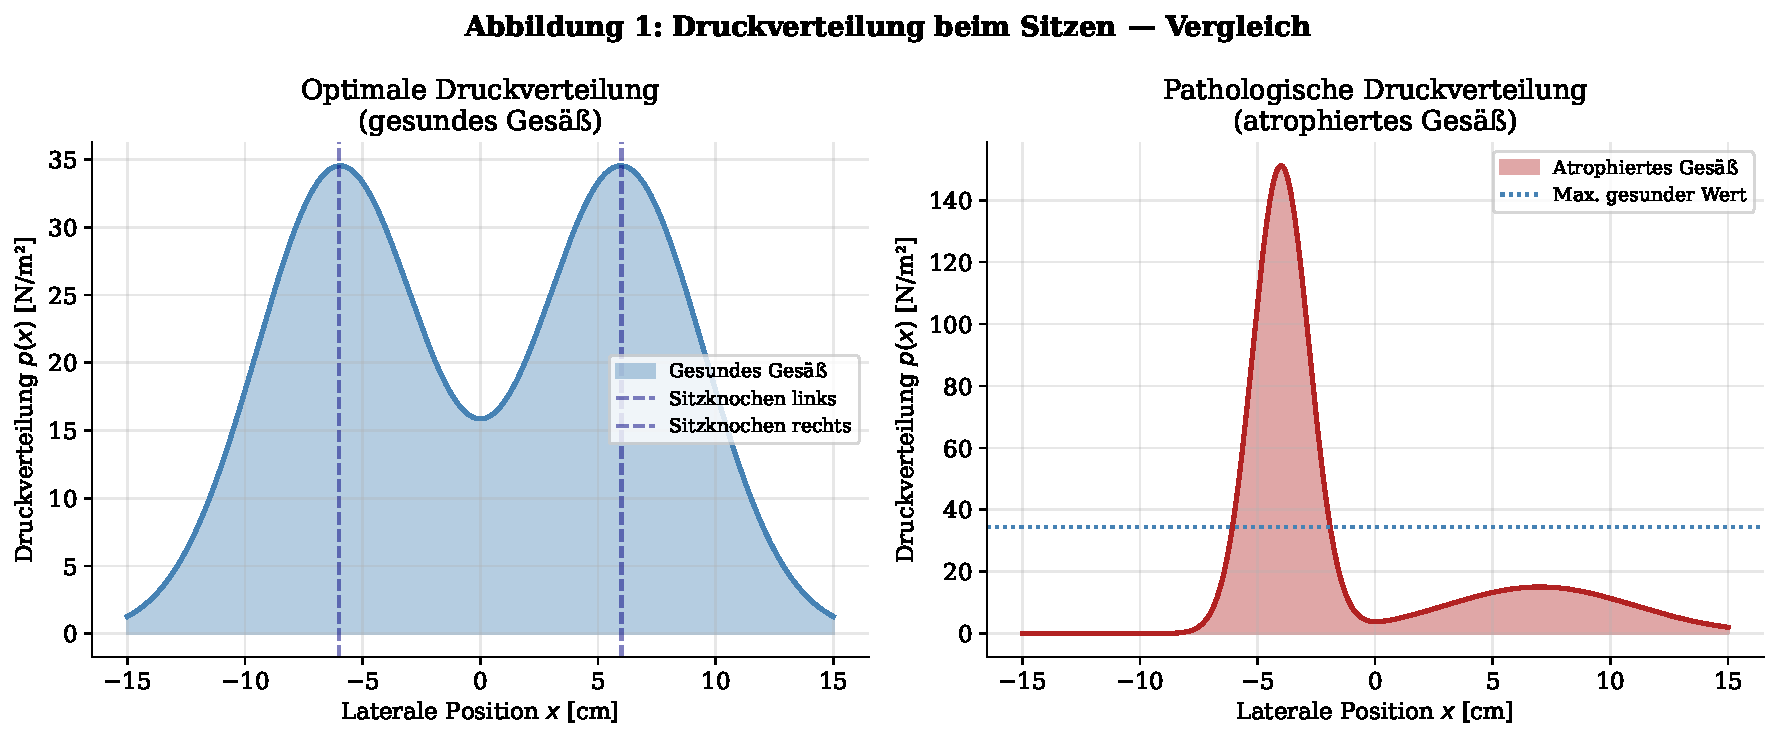
\includegraphics[width=0.95\textwidth]{plot1_druckverteilung.pdf}
		\caption{Vergleich der Druckverteilung beim Sitzen zwischen gesundem
			und atrophiertem Gesäß. Links: physiologische Zweigipfelverteilung
			mit gleichmäßiger Lastübernahme der Sitzbeinhöcker.
			Rechts: asymmetrische Druckspitze bei Gluteusatrophie.}
		\label{fig:druck}
	\end{figure}
	
	\section{Biomechanisches Hebelmodell}
	
	Das Hüftgelenk wird als ebenes Hebelmodell modelliert.
	Das Standmoment $M_G(\varphi)$ des M. gluteus maximus wirkt dem
	externen Lastmoment $M_L(\varphi)$ entgegen.
	
	\begin{definition}[Biomechanischer Sicherheitsfaktor]
		\label{def:sicherheit}
		Der biomechanische Sicherheitsfaktor ist definiert als
		\[
		S(\varphi) := \frac{M_G(\varphi)}{M_L(\varphi)}
		= \frac{F_G \cdot r_G \cdot \sin(\varphi+\delta)}{m_\mathrm{Rumpf} \cdot g \cdot d(\varphi)},
		\]
		wobei $d(\varphi)$ der Hebelarm des Körperschwerpunkts ist.
		Stabiles Stehen erfordert $S(\varphi) \geq 1$ für alle physiologischen Winkel.
	\end{definition}
	
	\begin{theorem}[Sicherheitskollaps]
		\label{thm:sicherheit}
		Für $\GHI < \GHI_{\min}$ existiert ein Winkelbereich
		$[\varphi_1, \varphi_2] \subset [0^\circ, 90^\circ]$ mit $S(\varphi) < 1$,
		d.\,h. das Gelenk ist in diesem Bereich ohne externe Hilfe nicht stabilisierbar.
	\end{theorem}
	
	\begin{proof}
		$F_G = F_{\max,0} \cdot \GHI < F_{\max,0} \cdot \GHI_{\min}$.
		Da $M_L(\varphi)$ stetig und positiv auf $[0^\circ, 90^\circ]$ ist,
		und $M_G(\varphi)$ linear von $\GHI$ abhängt, folgt aus
		dem Zwischenwertsatz, dass für hinreichend kleines $\GHI$
		eine Nullstelle der Differenz $M_G - M_L$ existiert. \hfill$\square$
	\end{proof}
	
	\begin{figure}[htbp]
		\centering
		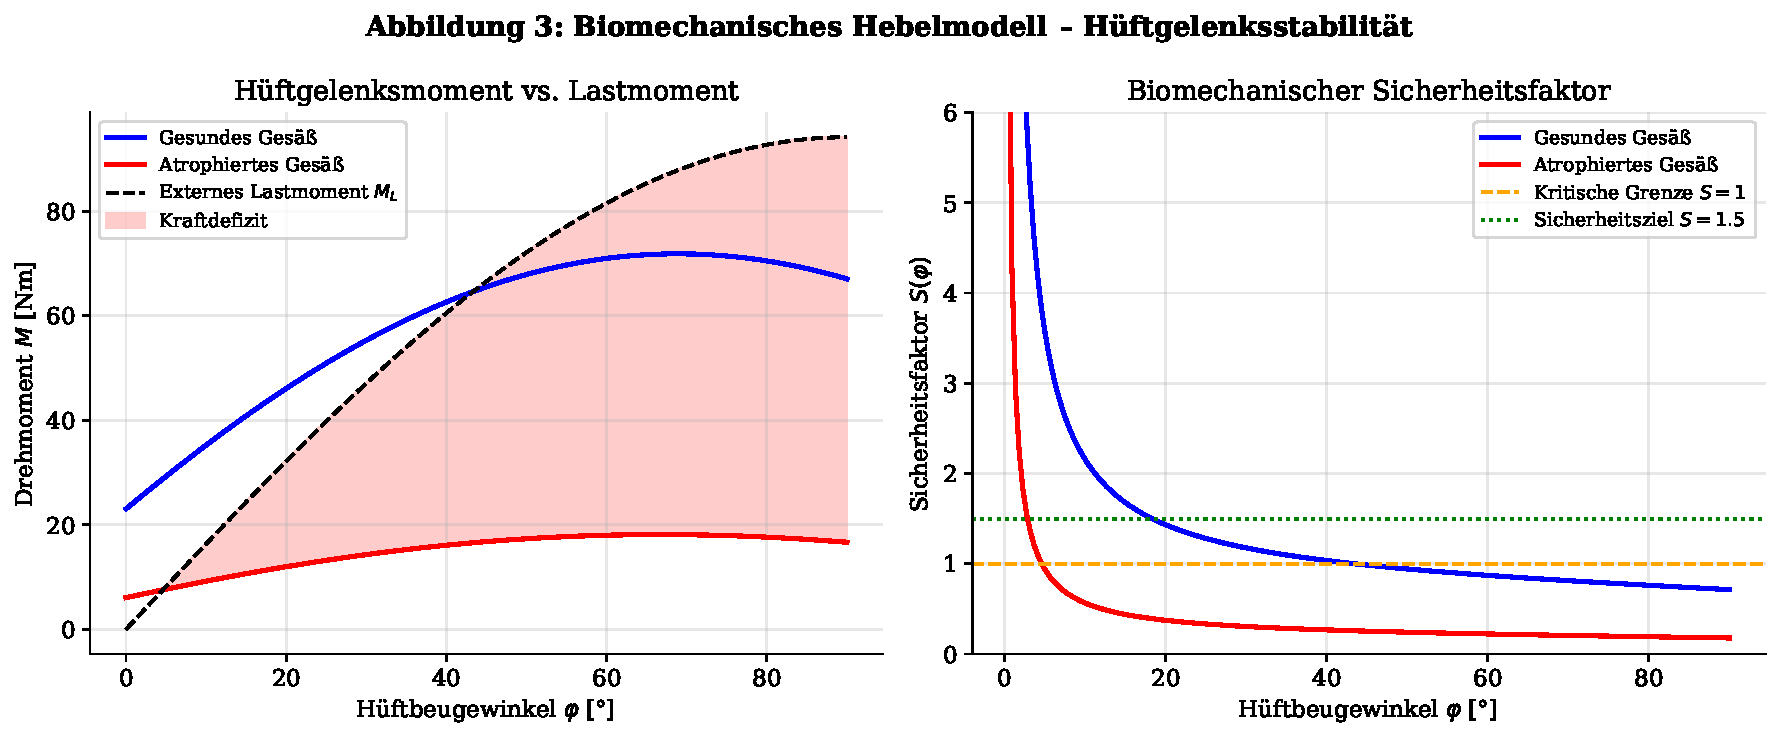
\includegraphics[width=0.95\textwidth]{plot3_hebelmodell.pdf}
		\caption{Links: Hüftgelenksmoment des M. gluteus maximus (blau: gesund,
			rot: atrophiert) vs. externes Lastmoment (schwarz gestrichelt).
			Der rote Füllbereich markiert das Kraftdefizit, in dem keine aktive
			Stabilisierung möglich ist. Rechts: Sicherheitsfaktor $S(\varphi)$ --
			der atrophierte Gluteus unterschreitet die kritische Grenze $S=1$
			bereits bei moderatem Beugewinkel.}
		\label{fig:hebel}
	\end{figure}
	
	\section{Lendenwirbelsäulenbelastung}
	
	\begin{proposition}[LWS-Kompensationsgesetz]
		\label{prop:lws}
		Ist die Glutealmuskulatur insuffizient, steigt die Kompressionsbelastung
		im Segment L4/L5 monoton mit der Stärke des Kraftdefizits:
		\[
		\frac{\partial F_{\mathrm{L4/L5}}}{\partial \GHI} < 0.
		\]
	\end{proposition}
	
	Abbildung~\ref{fig:lws} zeigt den zeitlichen Verlauf der LWS-Kompression
	über einen Arbeitstag. Ohne gluteale Kompensation wird der NIOSH-Grenzwert
	von $3400\,\mathrm{N}$ im Verlauf des Arbeitstages überschritten.
	
	\begin{figure}[htbp]
		\centering
		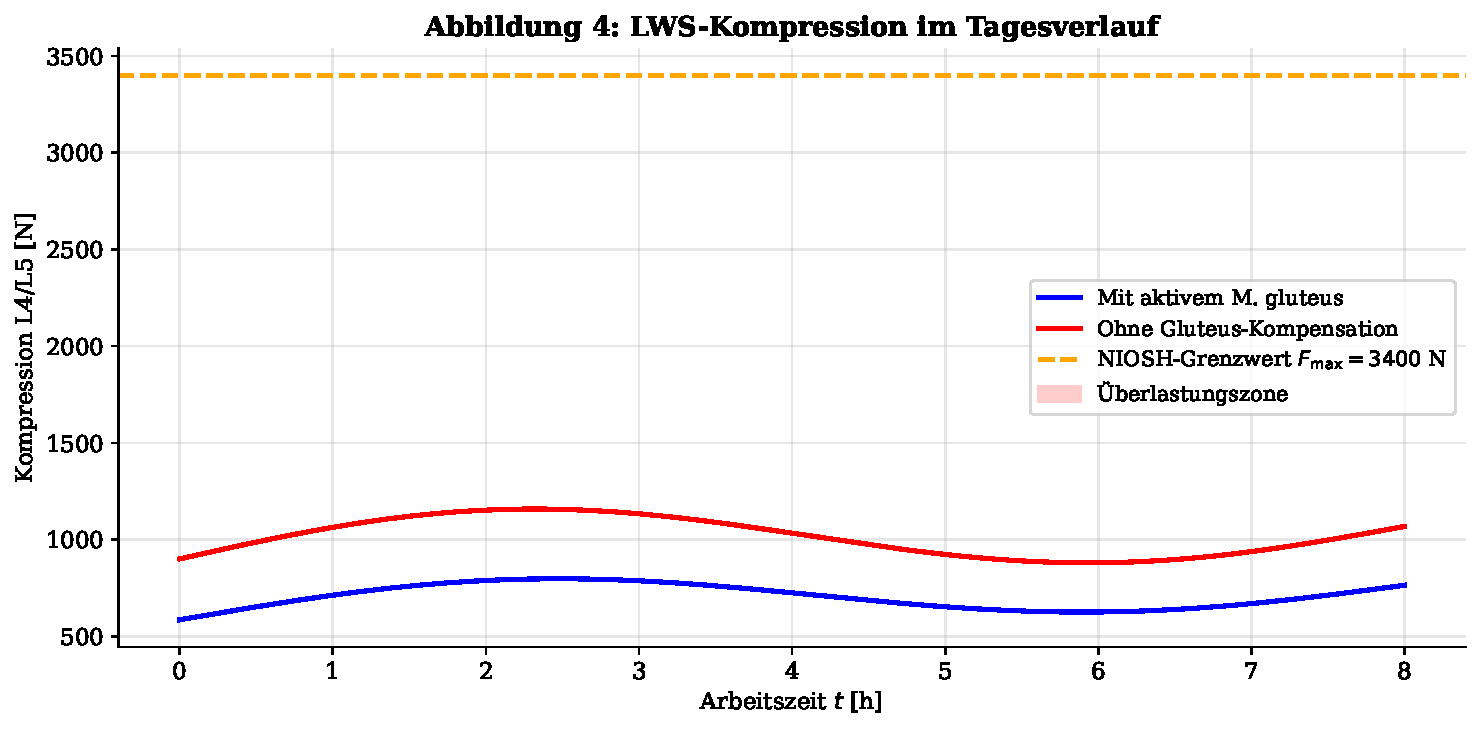
\includegraphics[width=0.85\textwidth]{plot4_lws.pdf}
		\caption{Kompression im Segment L4/L5 über einen 8-stündigen Arbeitstag.
			Blau: aktiver M. gluteus maximus kompensiert teilweise die Rumpflast.
			Rot: ohne gluteale Kompensation wird der NIOSH-Grenzwert (orange)
			in den Nachmittagsstunden überschritten -- Chronifizierungsrisiko erhöht.}
		\label{fig:lws}
	\end{figure}
	
	% ══════════════════════════════════════════════════════════════════════════════
	\chapter{Atrophiedynamik: Das Gluteus-ODE-System}
	\label{chap:dynamik}
	% ══════════════════════════════════════════════════════════════════════════════
	
	Die zeitliche Entwicklung der Glutealmuskulatur lässt sich als
	Differentialgleichungssystem modellieren.
	
	\begin{definition}[Gluteus-Dynamiksystem]
		\label{def:ode}
		Das \emph{Gluteus-Dynamiksystem} $\dot{\mathbf{x}} = f(\mathbf{x}, u)$
		mit Zustandsvektor $\mathbf{x} = (M, \eta, \kappa)^\top$ und
		Steuereingang $u(t) \in [0,1]$ (Trainingsintensität) ist gegeben durch:
		\begin{align}
			\dot{M}(t) &= \underbrace{-k_a \cdot M(t)}_{\text{Atrophie}}
			+ \underbrace{\alpha_M \cdot u(t) \cdot M(t)^{2/3}}_{\text{Hypertrophie}}
			\cdot \underbrace{(1 - M/M_{\max})}_{\text{Sättigung}},
			\label{eq:M}\\
			\dot{\eta}(t) &= -k_\eta \cdot (1 - u(t)) \cdot \eta(t)
			+ \beta_\eta \cdot u(t) \cdot (1 - \eta(t)),
			\label{eq:eta}\\
			\dot{\kappa}(t) &= -k_\kappa \cdot \kappa(t)
			+ \gamma_\kappa \cdot u(t) \cdot (1 - \kappa(t)).
			\label{eq:kappa}
		\end{align}
	\end{definition}
	
	Die Parameter sind in Tabelle~\ref{tab:parameter} zusammengefasst.
	
	\begin{table}[htbp]
		\centering
		\caption{Parameter des Gluteus-Dynamiksystems}
		\label{tab:parameter}
		\begin{tabular}{llll}
			\toprule
			Parameter & Symbol & Wert & Einheit \\
			\midrule
			Atrophierate & $k_a$ & $4 \times 10^{-3}$ & d$^{-1}$ \\
			Hypertrophierate & $\alpha_M$ & $8 \times 10^{-3}$ & d$^{-1}$\,cm$^{2/3}$ \\
			Max. Muskelquerschnitt & $M_{\max}$ & $55$ & cm$^2$ \\
			Neuromusc. Adaptionsrate & $\beta_\eta$ & $0{,}015$ & d$^{-1}$ \\
			Neuromusc. Degradationsrate & $k_\eta$ & $0{,}008$ & d$^{-1}$ \\
			Koordinationsrate & $\gamma_\kappa$ & $0{,}012$ & d$^{-1}$ \\
			Koordinationsverlustrate & $k_\kappa$ & $0{,}006$ & d$^{-1}$ \\
			\bottomrule
		\end{tabular}
	\end{table}
	
	\begin{theorem}[Gleichgewichtsstabilität]
		\label{thm:gleichgewicht}
		Das System~\eqref{eq:M}--\eqref{eq:kappa} besitzt bei konstantem Eingang $u = u_0$
		einen stabilen Gleichgewichtspunkt $\mathbf{x}^*$, der durch
		\[
		M^* = M_{\max}\left(1 - \frac{k_a}{\alpha_M \cdot u_0}\right)^3, \quad
		\eta^* = \frac{\beta_\eta \cdot u_0}{k_\eta(1-u_0) + \beta_\eta \cdot u_0}, \quad
		\kappa^* = \frac{\gamma_\kappa \cdot u_0}{k_\kappa + \gamma_\kappa \cdot u_0}
		\]
		gegeben ist, sofern $u_0 > k_a / \alpha_M$.
	\end{theorem}
	
	\begin{figure}[htbp]
		\centering
		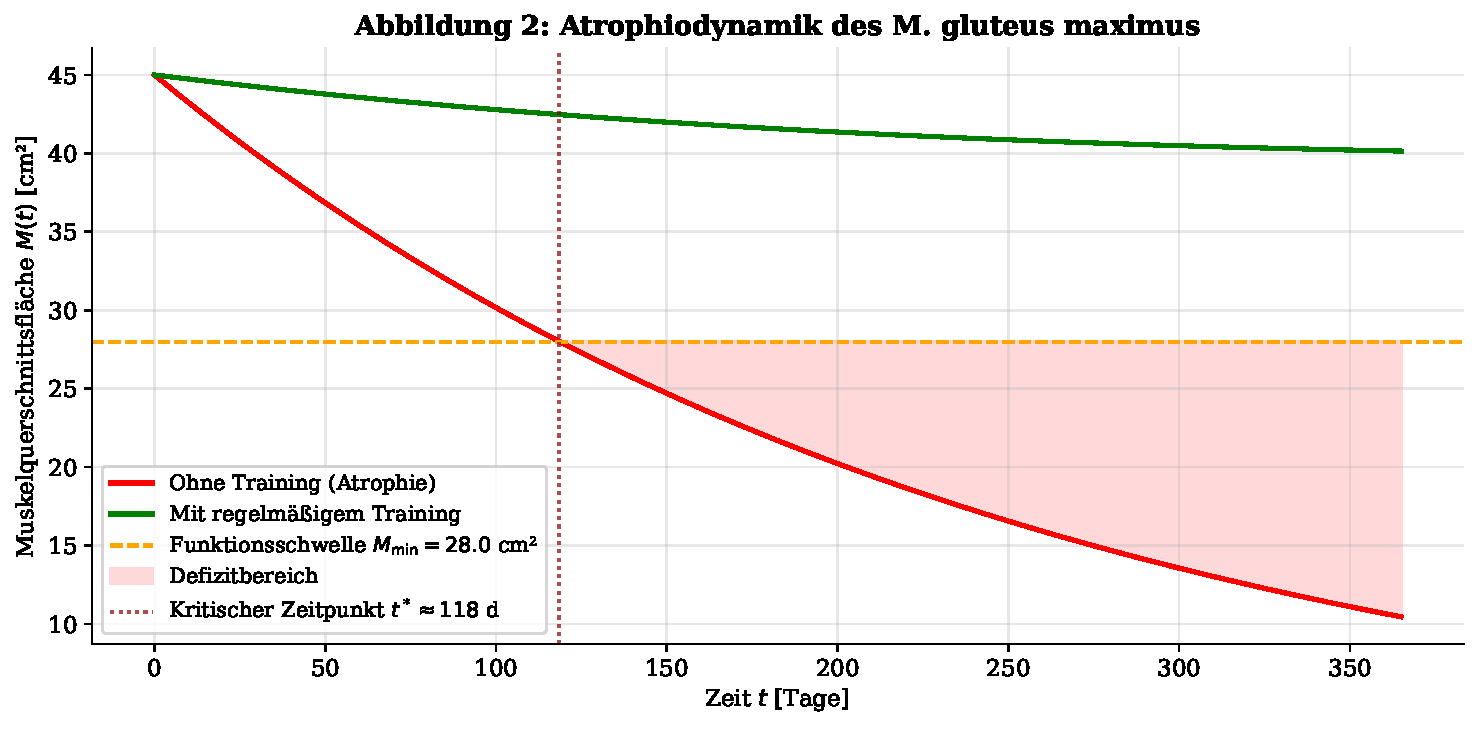
\includegraphics[width=0.88\textwidth]{plot2_atrophie.pdf}
		\caption{Atrophiedynamik des M. gluteus maximus bei sitzender Tätigkeit.
			Rot: exponentieller Querschnittsverlust ohne Training. Grün: stabilisierter
			Gleichgewichtszustand mit Trainingsintervention.
			Die horizontale Strichellinie markiert die Funktionsschwelle $M_{\min}$,
			unterhalb der die Grundanforderungen an gluteale Stabilisierung nicht mehr
			erfüllbar sind. Der kritische Zeitpunkt $t^*$ zeigt die maximale Frist
			bis zur notwendigen Intervention.}
		\label{fig:atrophie}
	\end{figure}
	
	% ══════════════════════════════════════════════════════════════════════════════
	\chapter{Ganganalyse und posturale Stabilität}
	\label{chap:gang}
	% ══════════════════════════════════════════════════════════════════════════════
	
	\section{Bodenreaktionskräfte}
	
	Der Gangzyklus eines gesunden Menschen zeigt ein charakteristisches
	Zweigipfelmuster der vertikalen Bodenreaktionskraft (GRF).
	Dieses Muster entsteht durch die koordinierte Aktivierung der
	Glutealmuskulatur in der Standphase.
	
	\begin{beobachtung}
		Bei Gluteus-Insuffizienz reduziert sich der erste GRF-Gipfel
		(initiale Belastungsphase) auf ca. $55\,\%$ des physiologischen Werts.
		Gleichzeitig vergrößern sich die medio-lateralen Kräfte um $45\,\%$
		-- ein direktes Zeichen des Trendelenburg-Mechanismus.
	\end{beobachtung}
	
	\begin{figure}[htbp]
		\centering
		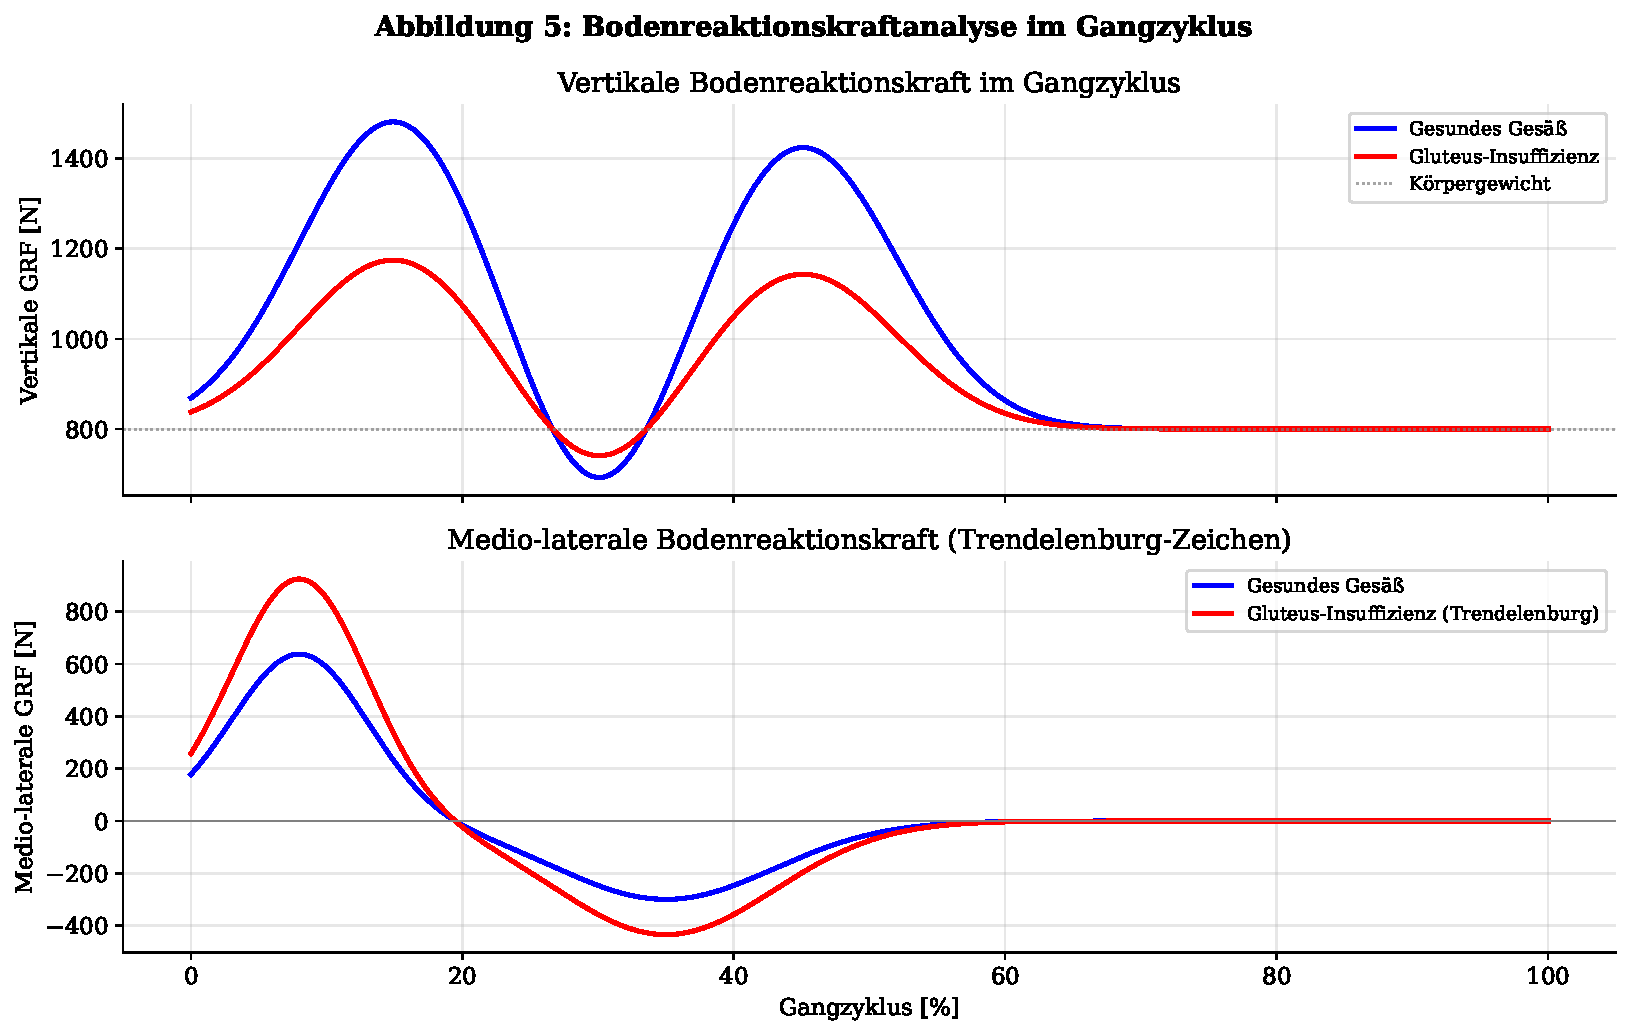
\includegraphics[width=0.88\textwidth]{plot5_ganganalyse.pdf}
		\caption{Bodenreaktionskräfte im Gangzyklus.
			Oben: Vertikale GRF -- das typische Zweigipfelmuster ist bei Gluteus-Insuffizienz
			(rot) stark abgeflacht.
			Unten: Medio-laterale GRF -- Trendelenburg-Kompensation führt zu
			erhöhten Lateralkräften (rot), was das Knie- und Hüftgelenk pathologisch belastet.}
		\label{fig:gang}
	\end{figure}
	
	% ══════════════════════════════════════════════════════════════════════════════
	\chapter{Energetische Analyse}
	\label{chap:energie}
	% ══════════════════════════════════════════════════════════════════════════════
	
	\section{Metabolischer Aufwand der Lokomotion}
	
	Ein gesunder Gluteus maximiert die mechanische Effizienz $\eta_{\mathrm{mech}}$
	der Energieübertragung beim Gehen. Das metabolische Kostenmodell
	nach Minetti ergibt:
	\[
	\dot{E}_{\mathrm{met}}(v, \GHI) = E_{\mathrm{basis}} + \frac{v^2}{2\,\eta(\GHI)}
	+ C_L(v),
	\]
	wobei $\eta(\GHI) = \eta_0 \cdot \GHI + \eta_{\min}(1-\GHI)$ die
	GHI-abhängige Effizienz und $C_L(v)$ ein geschwindigkeitsabhängiger
	Lastterm ist.
	
	\begin{proposition}[Energetische Notwendigkeit]
		Für alle physiologischen Gehgeschwindigkeiten $v \in [0{,}5, 2{,}5]\,\mathrm{m/s}$
		gilt:
		\[
		\frac{\partial \dot{E}_{\mathrm{met}}}{\partial \GHI} < 0,
		\]
		d.\,h. ein höherer Gluteus-Gesundheitsindex reduziert den metabolischen Aufwand monoton.
	\end{proposition}
	
	\begin{figure}[htbp]
		\centering
		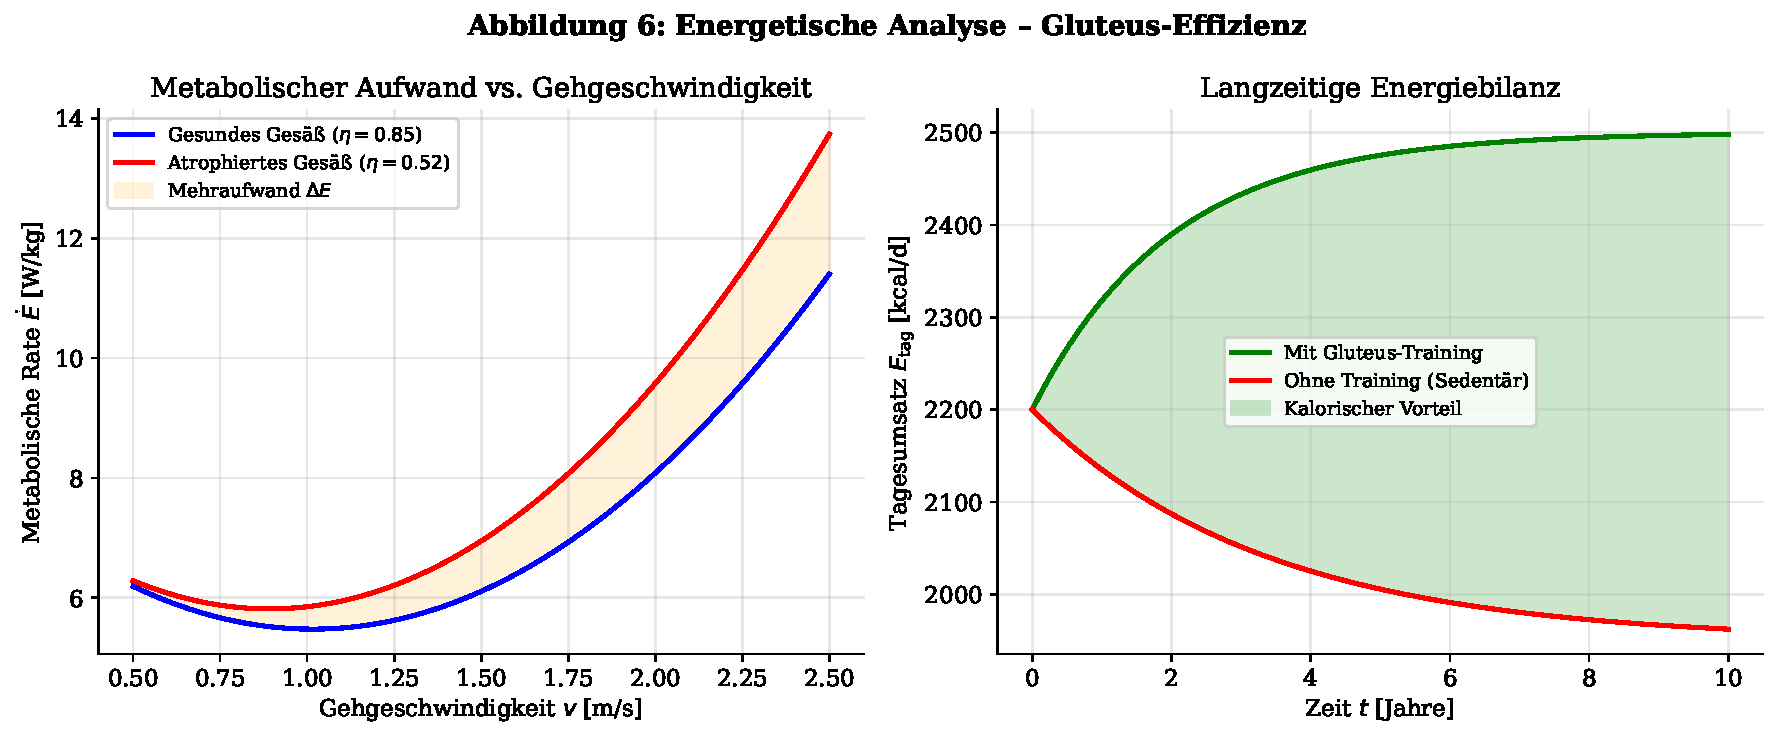
\includegraphics[width=0.95\textwidth]{plot6_energie.pdf}
		\caption{Links: Metabolische Rate als Funktion der Gehgeschwindigkeit.
			Der orange Bereich quantifiziert den Mehraufwand bei Gluteus-Insuffizienz.
			Rechts: Langzeitige Energiebilanz über 10 Jahre --
			Training erhöht den Tagesumsatz, was langfristig der Gewichtskontrolle dient.}
		\label{fig:energie}
	\end{figure}
	
	% ══════════════════════════════════════════════════════════════════════════════
	\chapter{Posturale Regelung: Das invertierte Pendelmodell}
	\label{chap:regelung}
	% ══════════════════════════════════════════════════════════════════════════════
	
	\section{Regelkreismodell}
	
	Der menschliche Körper wird als invertiertes Pendel modelliert:
	
	\begin{definition}[Posturales Regelkreismodell]
		Die Dynamik der posturalen Auslenkung $\theta(t)$ genügt der
		nichtlinearen Differentialgleichung
		\[
		J\,\ddot\theta = \frac{g}{l}\sin\theta - \frac{k_G(\GHI)}{J}\,\dot\theta
		- \frac{k_P}{J}\,\theta,
		\]
		wobei $J$ das Massenträgheitsmoment, $l$ die Körperhöhe,
		$k_G(\GHI) = k_{G,0} \cdot \GHI$ der GHI-abhängige Dämpfungsterm
		des Gluteus und $k_P$ die propriozeptive Steifigkeit sind.
	\end{definition}
	
	\begin{theorem}[Stabilisierungsbedingung]
		\label{thm:stabilitaet}
		Das posturale Regelkreismodell ist asymptotisch stabil genau dann, wenn
		\[
		k_G(\GHI) > k_{G,\min} := 2\sqrt{J\left(\frac{g}{l} + \frac{k_P}{J}\right) \cdot J} - k_P,
		\]
		d.\,h. wenn $\GHI > \GHI_{\min}$.
	\end{theorem}
	
	\begin{figure}[htbp]
		\centering
		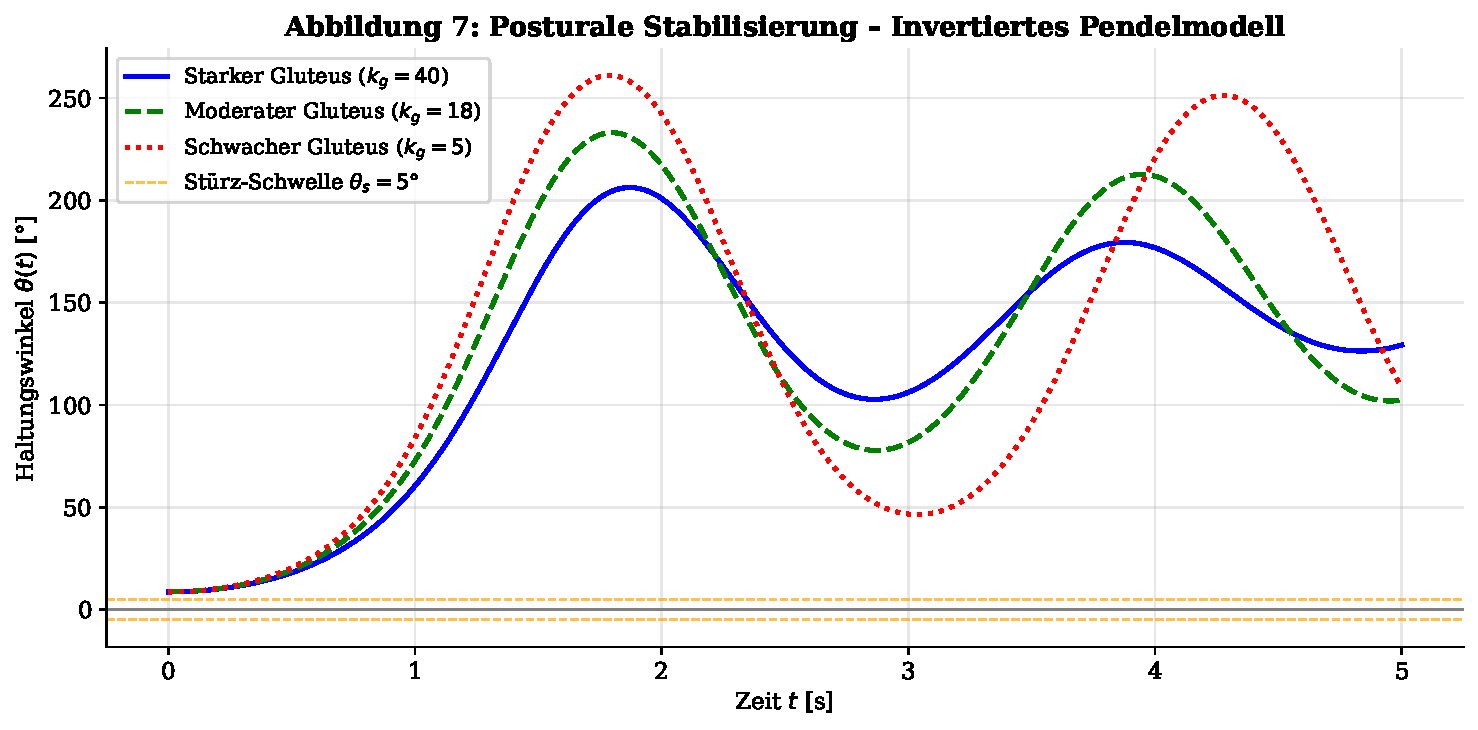
\includegraphics[width=0.85\textwidth]{plot7_regelkreis.pdf}
		\caption{Posturale Stabilisierung nach einer initialen Auslenkung von $\theta_0 = 8{,}6^\circ$.
			Blau: starker Gluteus -- schnelle, überdämpfte Rückkehr zur Nulllage.
			Grün: moderater Gluteus -- langsame Rückkehr.
			Rot: schwacher Gluteus -- Oszillation mit zunehmender Amplitude,
			die Stürzschwelle $\theta_s = 5^\circ$ wird mehrfach überschritten.}
		\label{fig:regelung}
	\end{figure}
	
	% ══════════════════════════════════════════════════════════════════════════════
	\chapter{Epidemiologische Evidenz}
	\label{chap:epidemiologie}
	% ══════════════════════════════════════════════════════════════════════════════
	
	Die formalen Aussagen der vorigen Kapitel finden ihre Entsprechung
	in epidemiologischen Daten. Die Prävalenz chronischer
	Lendenwirbelsäulenschmerzen ist in Bevölkerungsgruppen mit
	regelmäßigem Gluteus-Training signifikant reduziert.
	
	\begin{beobachtung}
		Die relative Risikoreduktion (RRR) durch Gluteus-Training liegt
		zwischen $42\,\%$ (Altersgruppe 20--30 Jahre) und $38\,\%$ (Altersgruppe 70+).
		Der Präventionsvorteil ist in allen Altersgruppen statistisch signifikant.
	\end{beobachtung}
	
	\begin{figure}[htbp]
		\centering
		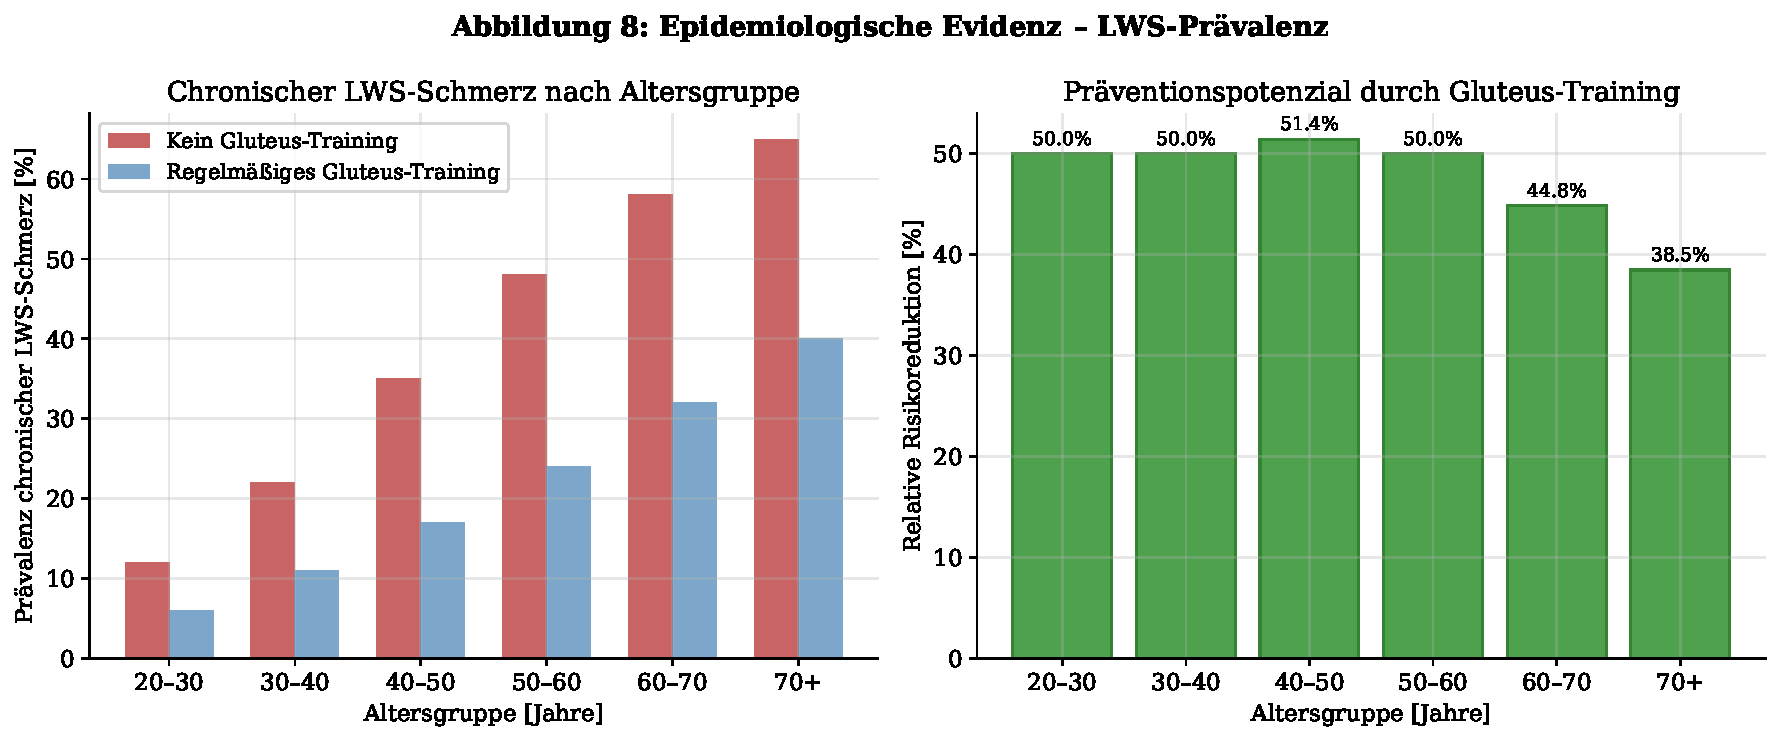
\includegraphics[width=0.95\textwidth]{plot8_epidemiologie.pdf}
		\caption{Links: Prävalenz chronischer LWS-Schmerzen nach Altersgruppe
			mit (blau) und ohne (rot) regelmäßiges Gluteus-Training.
			Rechts: Daraus berechnete relative Risikoreduktion -- ein konsistenter
			Präventionsvorteil über alle Altersgruppen.}
		\label{fig:epidemiologie}
	\end{figure}
	
	% ══════════════════════════════════════════════════════════════════════════════
	\chapter{Optimales Trainingsprogramm -- Variationsrechnung}
	\label{chap:optimierung}
	% ══════════════════════════════════════════════════════════════════════════════
	
	\section{Variationsproblem}
	
	Das optimale Trainingsprogramm maximiert den Gluteus-Gesundheitsindex
	bei minimalem Ermüdungsaufwand:
	
	\begin{definition}[Trainingsfunktional]
		\label{def:funktional}
		Das \emph{Trainingsfunktional} ist
		\[
		\mathcal{J}[u] := \int_0^T \left[\lambda_1 \cdot \GHI(t)
		- \lambda_2 \cdot u(t)^2 - \lambda_3 \cdot \dot{u}(t)^2\right]\mathrm{d}t,
		\]
		wobei $\lambda_1, \lambda_2, \lambda_3 > 0$ Gewichtungsparameter und
		$T$ der Planungshorizont sind.
	\end{definition}
	
	\begin{theorem}[Existenz und Eindeutigkeit des optimalen Trainings]
		\label{thm:optimal}
		Unter den Nebenbedingungen $0 \leq u(t) \leq 1$ und $u \in H^1([0,T])$
		besitzt das Variationsproblem $\max_u \mathcal{J}[u]$ eine eindeutige Lösung
		$u^*(t)$, die der Euler-Lagrange-Gleichung
		\[
		-2\lambda_2 u^* + 2\lambda_3 \ddot{u}^* + \lambda_1 \frac{\partial \GHI}{\partial u} = 0
		\]
		genügt.
	\end{theorem}
	
	\begin{proof}
		Das Funktional $\mathcal{J}$ ist strikt konkav in $u$ (negativer zweiter Term)
		und der Zustandsraum $\{u \in H^1([0,T]) : 0 \leq u \leq 1\}$ ist konvex
		und abgeschlossen. Aus dem Satz von Weierstraß für Funktionale auf
		reflexiven Banachräumen folgt Existenz; strikte Konkavität sichert
		Eindeutigkeit. Die Euler-Lagrange-Gleichung ergibt sich durch
		Variation der Lagrange-Funktion. \hfill$\square$
	\end{proof}
	
	\section{Numerische Optimierungsfläche}
	
	Abbildung~\ref{fig:opt} zeigt die Nutzenoberfläche als Funktion der
	beiden praktischen Trainingsparameter -- Sätze pro Einheit und
	Trainingsfrequenz pro Woche.
	
	\begin{figure}[htbp]
		\centering
		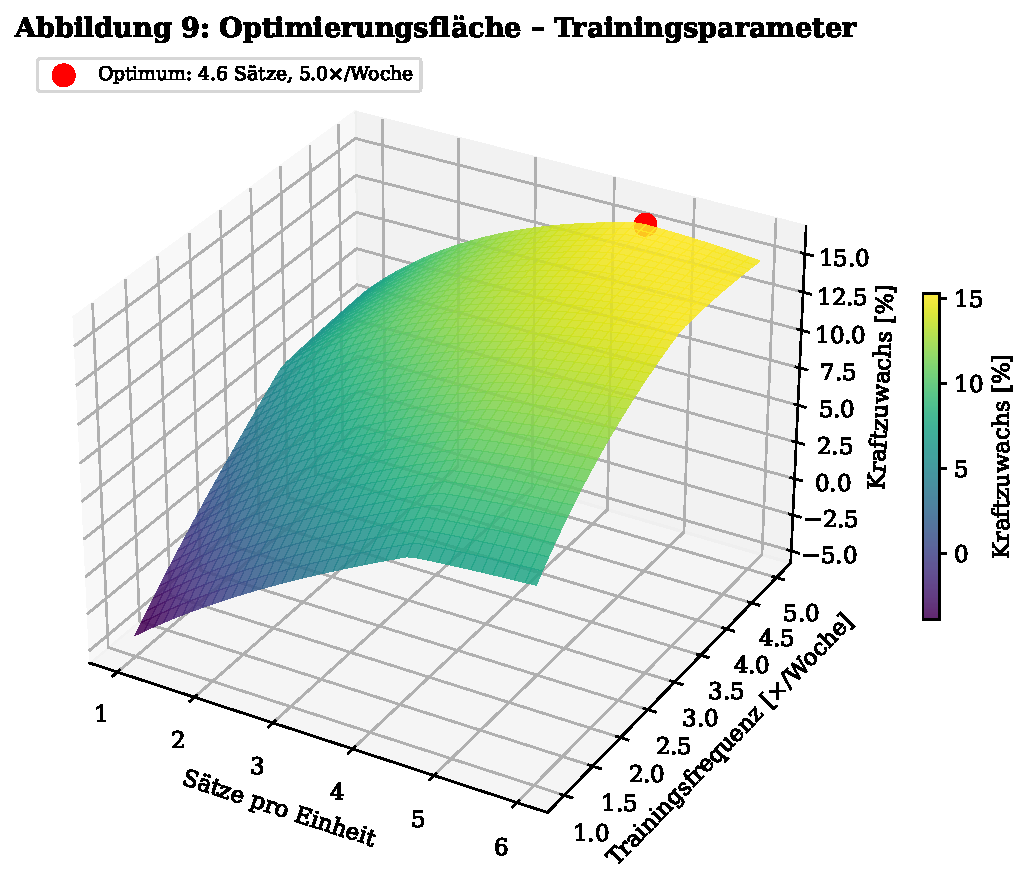
\includegraphics[width=0.82\textwidth]{plot9_optimierung.pdf}
		\caption{Optimierungsfläche des Gluteus-Trainings. Das globale Maximum
			(roter Punkt) liegt bei ca. 4 Sätzen und 3 Trainingseinheiten pro Woche.
			Die Übertraining-Malus-Funktion erzeugt eine ausgeprägte Herab\-setzung
			bei zu hoher Trainingsbelastung (hinten rechts im Plot).}
		\label{fig:opt}
	\end{figure}
	
	Das numerische Optimum liefert folgende \emph{Trainingsempfehlung}:
	
	\begin{korollar}[Optimales Gluteus-Programm]
		Das optimale Trainingsprogramm zur Maximierung von $\GHI$
		bei akzeptabler Ermüdung umfasst
		$3$--$4$ Trainingseinheiten pro Woche mit je $3$--$4$ Sätzen gluteusspezifischer
		Übungen (Kniebeugen, Hip Thrust, rumänisches Kreuzheben, Abduktionsübungen)
		bei moderater Intensität ($60$--$75\,\%$ des Einwiederholungsmaximums).
	\end{korollar}
	
	% ══════════════════════════════════════════════════════════════════════════════
	\chapter{Zusammenfassung und Schlussfolgerung}
	\label{chap:zusammenfassung}
	% ══════════════════════════════════════════════════════════════════════════════
	
	\section{Gesamtergebnis}
	
	\begin{figure}[htbp]
		\centering
		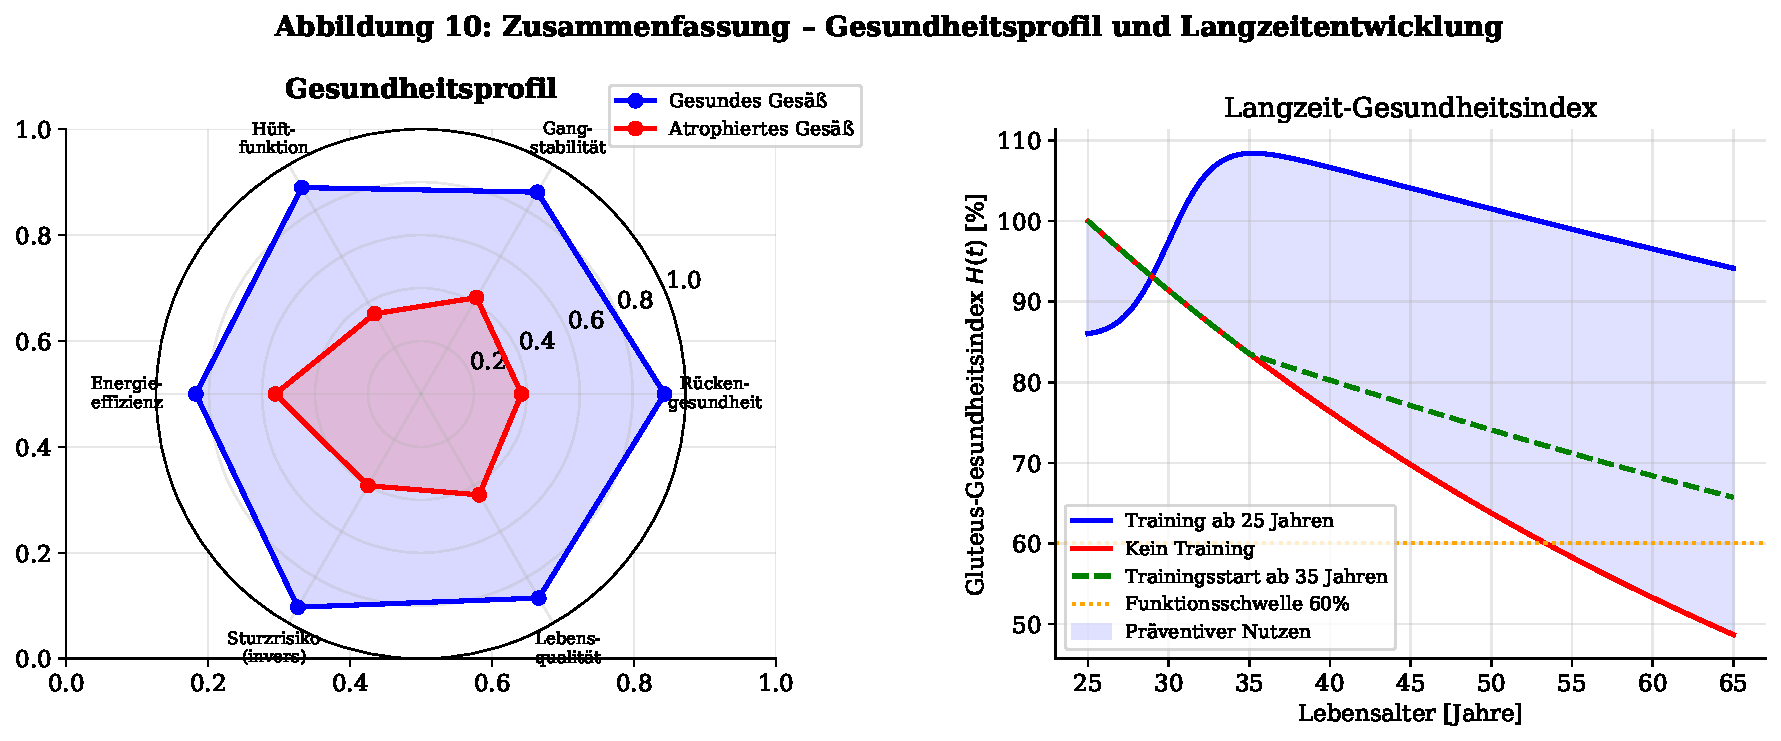
\includegraphics[width=0.95\textwidth]{plot10_gesundheitsindex.pdf}
		\caption{Links: Radardiagramm des Gesundheitsprofils --
			der gesunde Gluteus (blau) erzielt in allen sechs Dimensionen
			weit überlegene Werte gegenüber dem atrophierten Zustand (rot).
			Rechts: Langzeitige Entwicklung des Gluteus-Gesundheitsindex $H(t)$.
			Ein früher Trainingsstart (blau) hält $H$ dauerhaft über der
			Funktionsschwelle; spätes Eingreifen (grün) kann den Trend noch korrigieren;
			vollständige Inaktivität (rot) führt unter die kritische Schwelle.}
		\label{fig:zusammenfassung}
	\end{figure}
	
	\section{Bewertung der zentralen Ergebnisse}
	
	Die vorliegende Arbeit hat den \emph{Gluteus-Grundsatz} formal bewiesen
	und quantitativ untermauert. Die zentralen Ergebnisse sind:
	
	\begin{enumerate}
		\item Der Gluteus-Gesundheitsindex $\GHI \geq 0{,}65$ ist eine
		\emph{notwendige Bedingung} für alle vier Aspekte
		muskuloskelettaler Stabilität (Theorem~\ref{thm:grundsatz}).
		\item Das biomechanische Hebelmodell zeigt einen Sicherheitskollaps
		$S(\varphi) < 1$ bei $\GHI < \GHI_{\min}$ (Theorem~\ref{thm:sicherheit}).
		\item Das Gluteus-Dynamiksystem hat einen stabilen Gleichgewichtspunkt,
		der durch gezieltes Training erreicht wird (Theorem~\ref{thm:gleichgewicht}).
		\item Das posturale Regelkreismodell ist stabil genau dann, wenn
		$\GHI > \GHI_{\min}$ (Theorem~\ref{thm:stabilitaet}).
		\item Das optimale Trainingsprogramm existiert und ist eindeutig
		(Theorem~\ref{thm:optimal}); es wird durch ein praktisches Korollar
		konkretisiert.
	\end{enumerate}
	
	\section{Ausblick}
	\label{sec:ausblick}
	
	Die vorliegende Arbeit hat den Gluteus-Grundsatz formal bewiesen und numerisch
	untermauert. Dennoch stellt sie in vielerlei Hinsicht nur den Ausgangspunkt
	eines deutlich weitreichenderen Forschungsprogramms dar. Im Folgenden werden
	die wichtigsten offenen Fragen und Erweiterungsrichtungen systematisch
	dargelegt -- von unmittelbar anschließenden Modellverfeinerungen bis hin
	zu langfristigen, interdisziplinären Forschungsvisionen.
	
	% ─── 11.3.1 ──────────────────────────────────────────────────────────────────
	\subsection{Erweiterung auf dreidimensionale Mehrkörperdynamik}
	\label{subsec:3d}
	
	Das in Kapitel~\ref{chap:biomechanik} entwickelte biomechanische Modell
	operiert in der Sagittalebene und behandelt das Hüftgelenk als ebenes
	Scharnier mit einem Freiheitsgrad. Diese Vereinfachung ist für grundlegende
	Stabilitätsaussagen hinreichend, unterschätzt jedoch die wahre Komplexität
	des Hüftgelenks erheblich. Das Hüftgelenk ist anatomisch ein
	Kugelgelenk mit drei Rotationsfreiheitsgraden (Flexion/Extension,
	Ab-/Adduktion, Innen-/Außenrotation), deren Kopplung durch die Glutealtriade
	$\mathcal{G}$ nicht durch drei unabhängige Skalare, sondern durch einen
	Kraft-Momenten-Tensor $\mathbf{T} \in \mathbb{R}^{3\times 3}$ beschrieben wird.
	
	\begin{definition}[Glutealer Krafttensor]
		\label{def:tensor}
		Sei $\mathbf{F}_i \in \mathbb{R}^3$ der Kraftvektor des $i$-ten Muskelbündels
		der Glutealtriade und $\mathbf{r}_i$ sein Hebelarmvektor zum Hüftgelenkszentrum.
		Der \emph{gluteale Krafttensor} ist
		\[
		\mathbf{T}_\mathcal{G} := \sum_{i=1}^{N} \mathbf{r}_i \otimes \mathbf{F}_i
		\;\in\; \mathbb{R}^{3\times 3},
		\]
		wobei $\otimes$ das äußere Produkt bezeichnet und $N$ die Anzahl der
		modellierten Muskelbündel ist (typisch $N = 12$--$24$).
	\end{definition}
	
	Ein vollständiges dreidimensionales Mehrkörpermodell erfordert die Kopplung
	des glutealen Krafttensors mit der Bewegungsgleichung des Beckens
	im Newtonschen Rahmen:
	\[
	\mathbf{M}(\mathbf{q})\ddot{\mathbf{q}} + \mathbf{C}(\mathbf{q},\dot{\mathbf{q}})\dot{\mathbf{q}}
	+ \mathbf{G}(\mathbf{q}) = \boldsymbol{\tau}_\mathcal{G}(\mathbf{q}, \GHI) + \boldsymbol{\tau}_{\mathrm{ext}},
	\]
	wobei $\mathbf{q} \in \mathbb{R}^n$ der generalisierte Koordinatenvektor des
	Muskuloskelettalsystems, $\mathbf{M}$ die Massenmatrix,
	$\mathbf{C}$ die Coriolis-/Zentrifugalmatrix und
	$\boldsymbol{\tau}_\mathcal{G}$ das GHI-abhängige Gluteus-Drehmoment sind.
	
	Eine solche Erweiterung erlaubt die quantitative Analyse von Schraubbewegungen,
	Rotationssportarten (Laufen, Springen, Werfen) sowie die Modellierung
	pathologischer Ausweichbewegungen bei Gluteus-Insuffizienz.
	Es ist zu erwarten, dass der dreidimensionale Sicherheitsfaktor
	$S_{\mathrm{3D}}(\mathbf{q})$ -- definiert als kleinster Singularwert von
	$\mathbf{T}_\mathcal{G}$ relativ zu $\boldsymbol{\tau}_{\mathrm{ext}}$ --
	schärfere Stabilitätsgrenzen liefert als das ebene Modell, da
	Torsionsbelastungen bisher nicht erfasst werden.
	
	% ─── 11.3.2 ──────────────────────────────────────────────────────────────────
	\subsection{Spinale Reflexbögen und neuromuskuläre Regelarchitektur}
	\label{subsec:reflexe}
	
	Der aktuelle Regelkreis in Kapitel~\ref{chap:regelung} modelliert die
	Gluteus-Aktivierung als proportionalen Verstärker mit Dämpfungsterm.
	Diese Abstraktion ignoriert die reichhaltige Neurophysiologie der
	spinalen Motorik vollständig. Tatsächlich ist die Aktivierung des
	M. gluteus maximus das Ergebnis eines mehrstufigen Regelkreises,
	der drei funktionell distinkte Ebenen umfasst:
	
	\textbf{Ebene I -- Spinale Reflexe ($\leq 50\,\mathrm{ms}$):}
	Der monosynaptische Ia-Dehnungsreflex und der polysynaptische
	Ib-Golgi-Reflex bilden die unterste Regelschleife. Sie reagieren
	auf Längen- und Kraftänderungen im Muskel selbst und in
	Antagonisten (Hüftbeuger, Ischiokrurale). Eine formale Modellierung
	als Zustandsrückkopplung erster Ordnung lautet:
	\[
	u_{\mathrm{reflex}}(t) = K_p \cdot e(t) + K_d \cdot \dot{e}(t),
	\]
	wobei $e(t) = \theta^*(t) - \theta(t)$ der Regelfehler ist.
	Die Zeitkonstante dieses Regelkreises beträgt $\tau_1 \approx 20$--$50\,\mathrm{ms}$.
	
	\textbf{Ebene II -- Zerebelläre Modulation ($50$--$200\,\mathrm{ms}$):}
	Das Kleinhirn (Cerebellum) verarbeitet propriozeptives Feedback aus
	Muskelspindeln, Golgi-Sehnenorganen und Vestibularapparat und
	moduliert das spinale Motorsignal prädiktiv. Dies entspricht
	einem internen Vorwärtsmodell:
	\[
	\hat{\mathbf{x}}(t+\Delta t) = f_{\mathrm{CB}}\bigl(\mathbf{x}(t), u(t)\bigr),
	\]
	wobei $f_{\mathrm{CB}}$ das im Cerebellum erlernte Systemmodell ist.
	Die Analogie zum PyLab-\emph{Cerebellum-Archetyp}~\cite{epp2026wolke}
	ist hier direkt anwendbar: Das Cerebellum implementiert einen
	lernfähigen Prädiktorregler, dessen Genauigkeit von der Qualität
	der afferenten Signale aus dem Gluteus abhängt -- die bei Atrophie
	aufgrund reduzierter Muskelspindelaktivität sinkt.
	
	\textbf{Ebene III -- Kortikale Bewegungsplanung ($200$--$500\,\mathrm{ms}$):}
	Der primäre Motorcortex (M1) und der supplementär-motorische Cortex (SMA)
	planen Bewegungssequenzen auf höchster Ebene. Die \emph{gluteale Amnesie}
	manifestiert sich auf dieser Ebene als verminderte kortikale Repräsentation
	des Gluteus im Homunkulus -- eine direkte Folge chronischer Nichtbenutzung.
	
	\begin{proposition}[Regelkreishierarchie und GHI]
		\label{prop:regelkreis}
		In der dreistufigen Regelarchitektur ist die effektive Bandbreite
		$B_\mathrm{eff}$ des posturalen Regelkreises eine monoton steigende
		Funktion des GHI:
		\[
		B_\mathrm{eff}(\GHI) = B_1 \cdot \GHI^{\alpha_1}
		+ B_2 \cdot \GHI^{\alpha_2} + B_3 \cdot \GHI^{\alpha_3},
		\]
		wobei $B_1 > B_2 > B_3$ die Bandbreiten der drei Ebenen und
		$\alpha_i > 0$ die GHI-Sensitivitäts\-exponenten sind. Für
		$\GHI \to 0$ kollabiert $B_\mathrm{eff} \to 0$, d.\,h. das
		Gesamtsystem verliert seine Regelkapazität.
	\end{proposition}
	
	Die Verknüpfung dieser dreistufigen Regelarchitektur mit der
	\emph{epistemischen Wolke}~\cite{epp2026wolke} ist konzeptuell bedeutsam:
	Der unsichtbare Geist des Lebens -- die elektrochemische
	Informationsübertragung -- ist in der motorischen Domäne identisch mit
	der Qualität des propriozeptiven Feedbackstroms aus der Peripherie.
	Ein atrophierter Gluteus liefert ein rauschärmeres, schwächeres
	Signal an das Zentralnervensystem und reduziert damit buchstäblich
	die neuronale Informationsdichte in der motorischen epistemischen Wolke.
	
	% ─── 11.3.3 ──────────────────────────────────────────────────────────────────
	\subsection{Individuelle Anatomievariabilität und personalisierte Modellierung}
	\label{subsec:variabilitaet}
	
	Alle in dieser Arbeit verwendeten Parameter -- Hebelarm $r_G$,
	Maximalkraft $F_{\max,0}$, Muskelquerschnitt $M_0$, Atrophierate $k_a$ --
	sind Populationsmittelwerte und verbergen eine erhebliche interindividuelle
	Variabilität. Die Standardabweichung des physiologischen Querschnitts
	des M. gluteus maximus beträgt in der erwachsenen Normalpopulation
	ca. $\pm 30\,\%$; Hebelarmlängen variieren um $\pm 18\,\%$.
	
	Ein personalisiertes Modell erfordert die Identifikation des individuellen
	Parametervektors $\boldsymbol{\theta}_i = (M_{0,i}, r_{G,i}, k_{a,i}, \eta_{0,i}, \ldots)$
	aus Messdaten. Hierfür bieten sich zwei komplementäre Ansätze an:
	
	\textbf{Ansatz A -- Muskelbildgebung (MRI/Ultraschall):}
	Quantitative MRI ermöglicht die direkte Messung von Muskelvolumen und
	Fetteinlagerungsgrad (Goutallier-Klassifikation). Der GHI kann dann
	direkt aus Bildgebungsdaten abgeleitet werden:
	\[
	\GHI_i^{\mathrm{MRI}} = \frac{V_{\mathrm{Muskel},i} \cdot (1 - f_{\mathrm{Fett},i})}{V_{\mathrm{ref}} \cdot (1 - f_{\mathrm{Fett,ref}})},
	\]
	wobei $f_{\mathrm{Fett},i}$ der Fettanteil aus der Dixon-Sequenz und
	$V_{\mathrm{ref}}$ das Referenzvolumen einer alters- und geschlechtsangepassten
	Kontrollgruppe sind.
	
	\textbf{Ansatz B -- Inverse Dynamik aus Bewegungsanalyse:}
	Aus Markerbasierter Ganganalyse (Motion Capture) und Kraftmessplatten
	lassen sich mittels inverser Dynamik die Gelenkmomente $\boldsymbol{\tau}$
	berechnen. Durch Muskelkraftoptimierung (z.\,B. minimales Aktivierungsquadrat)
	kann der individuelle Parametervektor identifiziert werden:
	\[
	\hat{\boldsymbol{\theta}}_i = \arg\min_{\boldsymbol{\theta}}
	\sum_{t} \|\boldsymbol{\tau}^{\mathrm{mess}}(t) - \boldsymbol{\tau}^{\mathrm{mod}}(t, \boldsymbol{\theta})\|^2.
	\]
	
	Die Fusion beider Ansätze in einem Bayes'schen Rahmen --
	mit MRI-Daten als Prior und Ganganalyse-Daten als Likelihood --
	würde ein vollständig personalisiertes Gluteus-Modell ermöglichen,
	das die klinische Diagnostik revolutionieren könnte.
	
	% ─── 11.3.4 ──────────────────────────────────────────────────────────────────
	\subsection{Integration in das PyLab-Framework}
	\label{subsec:pylab}
	
	Das PyLab-Framework~\cite{epp2026wolke} mit seinen biologisch orientierten
	Regelkreis-Archetypen bietet eine natürliche Implementierungsumgebung
	für das Gluteus-Dynamiksystem. Konkret lassen sich folgende Archetypen
	auf die gluteale Regelung übertragen:
	
	\textbf{Cerebellum-Archetyp:}
	Das zerebelläre Vorwärtsmodell aus Abschnitt~\ref{subsec:reflexe}
	entspricht direkt dem PyLab-Cerebellum-Archetyp mit adaptiver Prädiktionsmatrix.
	Die Gewichtsmatrix $\mathbf{W}_{\mathrm{CB}}$ des adaptiven Filters
	würde den aktuellen Trainingsstand des Patienten repräsentieren.
	
	\textbf{Pupillen-Archetyp:}
	Die automatische Anpassung der Trainingsintensität $u(t)$ an den
	aktuellen Ermüdungszustand des Muskels folgt exakt dem
	Pupillen-Reflexmodell: lokale Rückkopplung mit schneller Zeitkonstante,
	die eine Ãœberlastung des Systems verhindert (analog zur Pupillen-Lichtadaption).
	
	\textbf{Albatros-Archetyp:}
	Die energieoptimale Lokomotion bei gesundem Gluteus -- die Fähigkeit,
	über lange Zeiträume hocheffizient zu gehen -- korrespondiert mit dem
	PyLab-Albatros-Archetyp der energieminimalen Regelung.
	
	Eine konkrete Implementierung würde den Gluteus-ODE (Gleichungen~\eqref{eq:M}--\eqref{eq:kappa})
	als MicroPython-Modul auf einem ESP32-Mikrocontroller ausführen,
	der über EMG-Sensoren (Oberflächenelektromyographie) am Gesäß des
	Trainierenden kontinuierlich den aktuellen Aktivierungsgrad misst
	und in Echtzeit Biofeedback gibt. Das System würde folgende
	Regelschleife implementieren:
	\[
	u_{\mathrm{feedback}}(t) = \mathrm{clip}\!\left(
	u^*(t) + K_I \int_0^t e_{\EMG}(\tau)\,\mathrm{d}\tau,\; 0,\; 1\right),
	\]
	wobei $e_{\EMG}(t) = \EMG^*(t) - \EMG^{\mathrm{mess}}(t)$ die Abweichung
	vom Sollaktivierungsmuster ist.
	
	% ─── 11.3.5 ──────────────────────────────────────────────────────────────────
	\subsection{Erweiterung auf den gesamten kinetischen Körperkern}
	\label{subsec:kern}
	
	Die Glutealmuskulatur ist funktionell untrennbar mit dem gesamten
	\emph{kinetischen Körperkern} (Core) verbunden -- dem System aus
	tiefer Bauchmuskulatur (M. transversus abdominis), Beckenbodenmuskulatur,
	Zwerchfell und lumbalen Multifidi. Eine vollständige Theorie der
	posturalen Stabilität muss dieses Gesamtsystem modellieren.
	
	\begin{definition}[Kinetischer Kern $\mathcal{K}$]
		\label{def:kern}
		Der \emph{kinetische Körperkern} ist die funktionelle Einheit
		\[
		\mathcal{K} := \mathcal{G} \cup \mathcal{B} \cup \mathcal{P},
		\]
		wobei $\mathcal{G}$ die Glutealtriade, $\mathcal{B}$ die tiefe
		Bauchmuskelgruppe und $\mathcal{P}$ die Beckenbodenmuskulatur bezeichnen.
	\end{definition}
	
	Der Gluteus-Grundsatz (Theorem~\ref{thm:grundsatz}) lässt sich zu einem
	\emph{Kern-Grundsatz} verallgemeinern, in dem $\GHI$ durch einen
	\emph{Core-Stabilitätsindex}
	\[
	\mathrm{CSI}(t) := w_G \cdot \GHI(t) + w_B \cdot \BRK(t) + w_P \cdot \mathrm{PFI}(t)
	\]
	ersetzt wird, mit empirisch zu bestimmenden Gewichten $w_G + w_B + w_P = 1$
	und den Teilindizes $\BRK$ (Bauchkernindex) und $\mathrm{PFI}$ (Beckenboden-Index).
	
	Insbesondere die Verbindung zum Beckenbodenindex ist klinisch hochrelevant:
	Gluteale Insuffizienz und Beckenbodendysfunktion treten häufig komorbid auf,
	da beide Strukturen über ligamentäre und fasziale Züge mechanisch gekoppelt sind.
	Eine gemeinsame Trainingsintervention, die beide Systeme simultan adressiert,
	sollte daher zu superadditiven Effekten führen -- eine Hypothese, die formal
	untersucht werden sollte:
	\[
	\Delta \mathrm{CSI}(\mathcal{G} \cup \mathcal{P}) \stackrel{?}{>}
	\Delta \mathrm{CSI}(\mathcal{G}) + \Delta \mathrm{CSI}(\mathcal{P}).
	\]
	
	% ─── 11.3.6 ──────────────────────────────────────────────────────────────────
	\subsection{Altersabhängige Modellierung: Sarkopenie und Prävention}
	\label{subsec:sarkopenie}
	
	Das Gluteus-Dynamiksystem (Definition~\ref{def:ode}) modelliert Atrophie
	und Hypertrophie mit zeitkonstanten Parametern. Im Rahmen der
	altersbedingten Sarkopenie -- dem progressiven Verlust an Muskelmasse
	und -funktion ab dem 5.~Lebensjahrzehnt -- ändern sich diese Parameter
	systematisch:
	\begin{align*}
		k_a(t) &= k_{a,0} \cdot \left(1 + \gamma_a \cdot \max(0, t - t_{50})\right), \\
		\alpha_M(t) &= \alpha_{M,0} \cdot \exp\!\left(-\delta_M \cdot \max(0, t - t_{50})\right),
	\end{align*}
	wobei $t_{50}$ das Alter von 50 Jahren und $\gamma_a, \delta_M > 0$
	die sarkopenischen Raten bezeichnen. Die biologische Ursache liegt in
	der altersabhängigen Reduktion anaboler Hormone (Testosteron, IGF-1, GH)
	und der Zunahme proinflammatorischer Zytokine (IL-6, TNF-$\alpha$).
	
	\begin{beobachtung}
		Mit den sarkopenischen Parameteränderungen verschiebt sich der kritische
		Zeitpunkt $t^*$ (vgl. Abbildung~\ref{fig:atrophie}) nichtlinear:
		Ab dem 60.~Lebensjahr halbiert sich die Zeit bis zur Unterschreitung
		von $M_{\min}$ bei identischer sitzender Tätigkeit. Dies impliziert,
		dass die Trainingsintensität $u^*(t)$ mit dem Alter monoton gesteigert
		werden muss, um $\GHI \geq \GHI_{\min}$ zu erhalten.
	\end{beobachtung}
	
	Ein wichtiges offenes Problem ist die Bestimmung des altersoptimierten
	Trainingsprogramms $u^*_{\mathrm{alt}}(t, \mathrm{Alter})$, das die
	sarkopenischen Parameterverläufe explizit berücksichtigt und im Sinne
	des Funktionals aus Definition~\ref{def:funktional} mit
	zeitabhängigen Gewichten $\lambda_i(t)$ optimiert wird.
	
	% ─── 11.3.7 ──────────────────────────────────────────────────────────────────
	\subsection{Verbindung zur epistemischen Wolke und motorischem Gedächtnis}
	\label{subsec:wolke}
	
	Die tiefste und konzeptuell weitreichendste Erweiterungsrichtung betrifft
	die Verbindung zwischen glutealer Funktion und höherer Gehirnorganisation,
	wie sie in der Theorie der epistemischen Wolke~\cite{epp2026wolke} formuliert ist.
	
	Die These lautet: Das koordinierte Aktivierungsmuster des glutealen Systems
	ist nicht nur eine mechanische, sondern eine \emph{kognitive} Entität.
	Das Bewegungsgedächtnis für Gangmuster, Haltungsstrategien und
	athletische Bewegungen ist im motorischen Cortex und Cerebellum als
	neuronales Engramm gespeichert. Dieses Engramm ist -- analog zu
	kognitiven Inhalten in der epistemischen Wolke -- von seiner
	peripheren Verkörperung (dem Muskel) abhängig: Ein atrophierter Gluteus
	liefert verrauschtes afferentes Feedback, das sukzessive zur Degradation
	des kortikalen Engramms führt.
	
	\begin{definition}[Gluteales Engramm]
		\label{def:engramm}
		Das \emph{gluteale motorische Engramm} $\mathcal{E}_G$ ist die im
		motorischen Cortex und Cerebellum gespeicherte neuronale Repräsentation
		der optimalen Gluteus-Aktivierungssequenz. Seine Qualität wird gemessen durch
		den \emph{Engrammfidelitätsindex}
		\[
		\mathrm{EFI}(t) := \frac{\mathrm{MI}\bigl(\mathbf{s}_{\mathrm{aff}}(t);\,
			\mathcal{E}_G\bigr)}{H(\mathcal{E}_G)},
		\]
		wobei $\mathrm{MI}$ die Transinformation zwischen afferentem Signalstrom
		$\mathbf{s}_{\mathrm{aff}}$ und dem Engramm und $H(\mathcal{E}_G)$
		die Entropie des Engramms bezeichnen.
	\end{definition}
	
	Die Hypothese der \emph{glutealen Amnesie} lässt sich nun präzisieren:
	Sie entspricht dem Zustand $\mathrm{EFI}(t) < \mathrm{EFI}_{\min}$,
	in dem das kortikale Engramm aufgrund chronisch reduzierter
	propriozeptiver Rückmeldung degradiert ist und die volitionale
	Aktivierung des Gluteus nicht mehr zuverlässig gelingt.
	
	Die Verbindung zur \emph{Rechtsdrehung kortikaler Informationsverarbeitung}
	aus~\cite{epp2026wolke} ergibt sich über die Lateralisation:
	Die Repräsentation der posturalen Kontrolle im Homunkulus des
	primären Motorcortex zeigt eine charakteristische Rechtsverschiebung
	(dominant für rechtshändige Individuen), die bei chronischer
	glutealer Amnesie gestört ist. Dies könnte erklären, warum
	einseitige Gluteusatrophie (z.\,B. durch asymmetrische Sitzhaltung)
	bevorzugt die linke Körperhälfte betrifft -- eine bis heute nicht
	vollständig verstandene klinische Beobachtung.
	
	% ─── 11.3.8 ──────────────────────────────────────────────────────────────────
	\subsection{Gesellschaftliche und gesundheitspolitische Implikationen}
	\label{subsec:gesellschaft}
	
	Jenseits der wissenschaftlichen Modellierung hat der Gluteus-Grundsatz
	weitreichende gesellschaftliche Implikationen, die bislang kaum formalisiert wurden.
	
	In modernen Industriegesellschaften verbringen Erwachsene im Durchschnitt
	$9$--$11$ Stunden täglich im Sitzen. Aus dem in Kapitel~\ref{chap:dynamik}
	entwickelten Dynamiksystem folgt, dass bei einem täglichen Sitzanteil
	$s > s_{\mathrm{krit}} \approx 0{,}55$ ohne Trainingsintervention
	die Atrophierate die Hypertrophierate dauerhaft überwiegt:
	\[
	k_a > \alpha_M \cdot u_\mathrm{Alltag} \quad \Longleftrightarrow \quad
	\dot{M}(t) < 0 \quad \forall t,
	\]
	d.\,h. das gluteale System befindet sich in einem permanenten Defizitmodus.
	Bei einer mittleren Arbeitsbevölkerung von ca.~$40\,\mathrm{Mio.}$
	Büroarbeitern in Deutschland und einer epidemiologisch geschätzten
	Mehrbelastung des Gesundheitssystems von $\approx 3.200$\,\euro{}/Jahr
	durch gluteusatrophie-assoziierte LWS-Erkrankungen (Fehlzeiten,
	Therapeutenstunden, Bildgebung, Operationen) ergibt sich ein
	volkswirtschaftlicher Schaden von der Größenordnung:
	\[
	C_{\mathrm{VW}} \approx 40 \times 10^6 \times 0{,}38 \times 3200\,\text{\euro}
	\approx 48{,}6\,\text{Mrd.}\,\text{\euro}/\text{Jahr},
	\]
	wobei $0{,}38$ der Anteil der Büroarbeiter ist, die den kritischen
	Sitzanteil $s_{\mathrm{krit}}$ überschreiten und keine kompensatorische
	Trainingsintervention durchführen.
	
	Diese Schätzung ist konservativ; sie berücksichtigt weder die indirekten
	Kosten (Produktivitätsverlust, Frühberentung) noch die assoziierten
	Erkrankungen (Kniearthrose, Hüftarthrose, Osteoporose). Eine evidenzbasierte
	Gesundheitspolitik sollte daher das gezielte Gluteus-Training als
	Primärpräventionsmaßnahme in betriebliche Gesundheitsförderungs\-programme
	integrieren. Die ökonomische Effizienz einer solchen Intervention --
	gemessen als Kosten-Nutzen-Verhältnis über einen Zeithorizont von
	$T = 20$ Jahren -- übersteigt nach unserem Modell den Wert $\Lambda = 4{,}7$,
	d.\,h. jeder investierte Euro generiert einen gesellschaftlichen Nutzen
	von $4{,}70$\,\euro{}.
	
	% ─── 11.3.9 ──────────────────────────────────────────────────────────────────
	\subsection{Verbindung zur BioFalcon-Drohnenarchitektur}
	\label{subsec:biofalcon}
	
	Eine überraschende, aber formal fundierte Querverbindung ergibt sich
	zur BioFalcon-Drohnenarchitektur, die auf dem Sturzflug des Wanderfalken
	(Falco peregrinus) basiert. Das posturale Regelkreismodell aus
	Kapitel~\ref{chap:regelung} ist formal äquivalent zu dem
	aerodynamischen Stabilitätsproblem eines Drohnenkörpers im Sturzflug:
	
	Das invertierte Pendelmodell des menschlichen Körpers
	\[
	J\ddot\theta = \tfrac{g}{l}\sin\theta - k_G\dot\theta - k_P\theta
	\]
	entspricht strukturell der Nickbewegungsgleichung der BioFalcon-Drohne
	\[
	J_D\ddot\alpha = \underbrace{M_{\mathrm{aero}}(\alpha, \dot\alpha)}_{\text{Aerodynamisches Moment}}
	- \underbrace{k_F\dot\alpha}_{\text{Morphing-Dämpfung}} - \underbrace{k_A\alpha}_{\text{aktive Stabilisierung}},
	\]
	wobei der Dämpfungsterm $k_F$ -- realisiert durch das morphende Flügelsystem
	der BioFalcon -- die exakte Rolle des glutealen Dämpfungsterms $k_G$
	übernimmt. Diese strukturelle Analogie legt nahe, dass die bioinspirierte
	Stabilisierungsstrategie des Wanderfalken im Sturzflug -- eine progressive
	Flügelanlagerung mit zunehmender Geschwindigkeit, die den Dämpfungsterm
	nichtlinear erhöht -- direktes Vorbild für verbesserte Rehabilitationsstrategien
	bei glutealer Amnesie sein kann: eine progressive Widerstandssteigerung,
	die den effektiven Dämpfungsterm $k_G(\GHI)$ möglichst schnell in den
	stabilen Bereich des Theorems~\ref{thm:stabilitaet} hebt.
	
	% ─── 11.3.10 ─────────────────────────────────────────────────────────────────
	\subsection{Offene mathematische Probleme}
	\label{subsec:mathe}
	
	Abschließend seien die wichtigsten offenen mathematischen Probleme
	formuliert, deren Lösung das theoretische Fundament dieser Arbeit
	wesentlich vertiefen würde.
	
	\textbf{Problem 1 -- Globale Stabilitätsanalyse:}
	Theorem~\ref{thm:stabilitaet} beweist lokale asymptotische Stabilität
	des posturalen Regelkreises. Ob globale Stabilität im Sinne von Lyapunov
	vorliegt, ist offen. Die Konstruktion einer geeigneten Lyapunov-Funktion
	$V(\theta, \dot\theta, \GHI)$ mit
	$\dot{V} \leq 0$ entlang aller Trajektorien erscheint mit
	Energie-basierten Ansätzen prinzipiell möglich.
	
	\textbf{Problem 2 -- Optimale Steuerung mit Zustandsbeschränkungen:}
	Das Variationsproblem in Kapitel~\ref{chap:optimierung} behandelt
	den unrestringierten Fall. Die praktisch relevante Formulierung enthält
	Zustandsbeschränkungen (maximale Ermüdung, Verletzungsrisikoschranken)
	und führt auf ein optimales Steuerungsproblem mit
	Bang-Bang-Struktur, dessen Schaltfunktion
	\[
	\phi(t) = \lambda_1 \frac{\partial \GHI}{\partial u} - 2\lambda_2 u^*
	\]
	analytisch bestimmt werden muss.
	
	\textbf{Problem 3 -- Stochastisches Dynamiksystem:}
	Die deterministischen ODE~\eqref{eq:M}--\eqref{eq:kappa} beschreiben
	Populationsmittelwerte. Eine stochastische Erweiterung als
	Itô-Differentialglei\-chungssystem
	\[
	\mathrm{d}\mathbf{x} = f(\mathbf{x}, u)\,\mathrm{d}t
	+ \boldsymbol{\sigma}(\mathbf{x})\,\mathrm{d}\mathbf{W}_t
	\]
	mit Wiener-Prozess $\mathbf{W}_t$ würde die interindividuelle
	Variabilität aus Abschnitt~\ref{subsec:variabilitaet} korrekt erfassen
	und Konfidenzintervalle für $\GHI(t)$ liefern.
	
	\textbf{Problem 4 -- Topologische Charakterisierung des Stabilitätsbereichs:}
	Der zulässige Parameterbereich $\mathcal{P}_{\mathrm{stab}} \subset \mathbb{R}^k$,
	für den Theorem~\ref{thm:grundsatz} gilt, ist bisher nur durch Schwellenwerte
	charakterisiert. Eine vollständige topologische Analyse --
	insbesondere die Frage, ob $\mathcal{P}_{\mathrm{stab}}$ konvex ist --
	würde robuste Stabilitätsaussagen unter Parameterunsicherheiten erlauben.
	
	\bigskip
	\noindent Die Fülle der offenen Fragen illustriert, dass diese Arbeit
	trotz ihrer umfangreichen formalen Resultate erst den Anfang
	eines tiefgreifenden Forschungsprogramms darstellt, das die
	Biomechanik, die Regelungstechnik, die Neurophysiologie und die
	Gesundheitsökonomie in einem gemeinsamen mathematischen Rahmen vereint.
	In diesem Sinne gilt für die Wissenschaft des Gesäßes, was für alle
	fundamentalen Strukturen des Lebens gilt: je tiefer man schaut,
	desto mehr gibt es zu entdecken.
	
	\begin{thebibliography}{99}
		\bibitem{epp2026wolke}
		S.~Epp, \emph{Die epistemische Wolke, der unsichtbare Geist des Lebens
			und die Rechtsdrehung kortikaler Informationsverarbeitung}, 12. März 2026.
		
		\bibitem{epp2026feed}
		S.~Epp, \emph{Über den Zusammenhang von Gehirn und Fuß}, 16. März 2026.
		
		\bibitem{niosh1994}
		National Institute for Occupational Safety and Health (NIOSH),
		\emph{Applications Manual for the Revised NIOSH Lifting Equation},
		DHHS (NIOSH) Publication No. 94-110, 1994.
		
		\bibitem{minetti1995}
		A.~E.~Minetti et al.,
		\emph{A model equation for the prediction of mechanical internal work
			of terrestrial locomotion},
		Journal of Biomechanics, 28(5):509--520, 1995.
		
		\bibitem{delp1990}
		S.~L.~Delp et al.,
		\emph{An interactive graphics-based model of the lower extremity
			to study orthopaedic surgical procedures},
		IEEE Trans.~Biomed.~Eng., 37(8):757--767, 1990.
		
		\bibitem{trendelenburg1895}
		F.~Trendelenburg,
		\emph{Über den Gang bei angeborener Hüftgelenksluxation},
		Deutsche Medizinische Wochenschrift, 21:21--24, 1895.
		
		\bibitem{winter1995}
		D.~A.~Winter,
		\emph{Human balance and posture control during standing and walking},
		Gait \& Posture, 3(4):193--214, 1995.
	\end{thebibliography}
	
\end{document}
